\documentclass[12pt,a4paper]{article}
\usepackage[a4paper, margin=0.8in, headheight=14pt]{geometry}
\usepackage{fontspec}
\usepackage{unicode-math}
\setmainfont{TeX Gyre Pagella}
\setmonofont[Scale=0.88]{TeX Gyre Cursor}
\setmathfont{Latin Modern Math}
\usepackage{xcolor}
\usepackage{colortbl}
\usepackage{titlesec}
\usepackage{enumitem}
\usepackage{tabularx}
\usepackage{booktabs}
\usepackage{array}
\usepackage{amsmath}
\usepackage{tikz}
\usetikzlibrary{shapes.geometric, arrows.meta, positioning, calc, fit, decorations.pathreplacing, decorations.pathmorphing}
\usepackage{tcolorbox}
\tcbuselibrary{skins, breakable}
\usepackage{hyperref}
\usepackage{fancyhdr}
\usepackage{graphicx}
\usepackage{microtype}
\hyphenpenalty=10000
\exhyphenpenalty=10000
\sloppy
\usepackage{caption}
\usepackage{setspace}
\usepackage{multirow}
\usepackage{tocloft}
\newcommand{\Q}[1]{\textbf{#1}\par\noindent\ignorespaces}
\definecolor{myred}{RGB}{196,30,58}
\definecolor{mydark}{RGB}{30,30,50}
\definecolor{mygreen}{RGB}{14,120,80}
\definecolor{myteal}{RGB}{0,130,140}
\definecolor{myamber}{RGB}{180,100,0}
\definecolor{mypurple}{RGB}{100,30,160}
\definecolor{mygray}{RGB}{246,247,249}
\definecolor{mgframe}{RGB}{180,185,200}
\definecolor{watermark}{RGB}{145,150,170}
\definecolor{hdrred}{RGB}{250,232,235}
\definecolor{hdrgreen}{RGB}{220,244,233}
\definecolor{hdrteal}{RGB}{220,242,244}
\definecolor{hdramber}{RGB}{253,242,215}
\definecolor{hdrpurple}{RGB}{238,228,255}
\definecolor{hdrgray}{RGB}{238,240,245}
\definecolor{rowalt}{RGB}{250,251,253}

\titleformat{\section}{\large\bfseries\color{myred}}{\thesection.}{0.5em}{}[\vspace{1pt}{\color{myred}\rule{\linewidth}{0.8pt}}]
\titleformat{\subsection}{\normalsize\bfseries\color{myteal}}{\thesubsection}{0.5em}{}
\titlespacing*{\section}{0pt}{18pt}{7pt}
\titlespacing*{\subsection}{0pt}{11pt}{4pt}
\setlength{\parindent}{0pt}
\setlength{\parskip}{4pt}
\renewcommand{\cfttoctitlefont}{\large\bfseries\color{myred}}
\renewcommand{\cftaftertoctitle}{\par\noindent{\color{myred}\rule{\linewidth}{0.8pt}}}
\setlength{\cftbeforetoctitleskip}{0pt}
\setlength{\cftaftertoctitleskip}{6pt}
\renewcommand{\cftsecfont}{\normalsize\bfseries\color{mydark}}
\renewcommand{\cftsecpagefont}{\normalsize\bfseries\color{mydark}}
\renewcommand{\cftsecleader}{\cftdotfill{\cftdotsep}}
\setlength{\cftbeforesecskip}{7pt}
\renewcommand{\cftsubsecfont}{\small\color{mydark}}
\renewcommand{\cftsubsecpagefont}{\small\color{mydark}}
\setlength{\cftbeforesubsecskip}{3pt}
\setlength{\cftsubsecindent}{1.4em}
\renewcommand{\cftpartfont}{\normalsize\bfseries\color{myteal}}
\renewcommand{\cftpartpagefont}{\normalsize\bfseries\color{myteal}}
\setlength{\cftbeforepartskip}{14pt}
\renewcommand{\arraystretch}{1.45}
\setlength{\tabcolsep}{6pt}
\arrayrulecolor{mydark}
\newcolumntype{B}[1]{>{\small\bfseries\raggedright\arraybackslash}m{#1}}
\newcolumntype{C}[1]{>{\centering\arraybackslash}m{#1}}
\newcolumntype{Y}{>{\small\raggedright\arraybackslash}X}
\renewcommand{\tabularxcolumn}[1]{m{#1}}
\newcommand{\currmodule}{Module 1}
\pagestyle{fancy}
\fancyhf{}
\fancyhead[L]{\small\color{myred}\textbf{PE-EC603C}\;\color{mydark}--- CMOS VLSI Design}
\fancyhead[R]{\small\color{myteal}\textbf{\currmodule\ Notes}}
\fancyfoot[C]{\small\color{mydark}\thepage}
\fancyfoot[R]{\small\color{watermark}\textit{\copyright\ Biraj}}
\renewcommand{\headrulewidth}{0.5pt}
\renewcommand{\footrulewidth}{0.3pt}

\hypersetup{colorlinks=true, linkcolor=myteal, urlcolor=myteal,
  pdfauthor={Biraj Sarkar},
  pdftitle={PE-EC603C --- Combined Notes}}

\tcbset{
  tikzbox/.style={
    colback=mygray, colframe=mgframe, boxrule=0.6pt, arc=4pt,
    left=8pt, right=8pt, top=6pt, bottom=6pt,
    colbacktitle=mgframe, coltitle=mydark,
    fonttitle=\small\bfseries
  },
  defbox/.style={
    colback=hdrgreen, colframe=mygreen, boxrule=0.8pt, arc=4pt,
    left=9pt, right=9pt, top=6pt, bottom=6pt,
    colbacktitle=mygreen, coltitle=white,
    fonttitle=\small\bfseries
  },
  formulabox/.style={
    colback=hdrteal, colframe=myteal, boxrule=0.8pt, arc=4pt,
    left=9pt, right=9pt, top=7pt, bottom=7pt,
    colbacktitle=myteal, coltitle=white,
    fonttitle=\small\bfseries
  },
  examplebox/.style={
    colback=hdramber, colframe=myamber, boxrule=0.8pt, arc=4pt,
    left=9pt, right=9pt, top=6pt, bottom=6pt,
    colbacktitle=myamber, coltitle=white,
    fonttitle=\small\bfseries
  },
  masonbox/.style={
    colback=hdrpurple, colframe=mypurple, boxrule=0.8pt, arc=4pt,
    left=9pt, right=9pt, top=6pt, bottom=6pt,
    colbacktitle=mypurple, coltitle=white,
    fonttitle=\small\bfseries
  },
  exambox/.style={
    colback=hdrpurple, colframe=mypurple, boxrule=1pt, arc=5pt,
    left=10pt, right=10pt, top=8pt, bottom=8pt,
    colbacktitle=mypurple, coltitle=white,
    fonttitle=\bfseries,
    breakable, title after break={\textbf{Frequently Asked / Viva Questions (contd.)}}}
}
\tcbset{breakable}
\tcbset{after={\color{black}}}

\tikzset{
  block/.style={rectangle, draw=myteal, fill=hdrteal,
    text width=2.4cm, align=center, minimum height=0.95cm,
    font=\small, rounded corners=3pt, line width=0.7pt},
  redblock/.style={rectangle, draw=myred, fill=hdrred,
    text width=2.4cm, align=center, minimum height=0.95cm,
    font=\small, rounded corners=3pt, line width=0.7pt},
  greenblock/.style={rectangle, draw=mygreen, fill=hdrgreen,
    text width=2.4cm, align=center, minimum height=0.95cm,
    font=\small, rounded corners=3pt, line width=0.7pt},
  amberblock/.style={rectangle, draw=myamber, fill=hdramber,
    text width=2.4cm, align=center, minimum height=0.95cm,
    font=\small, rounded corners=3pt, line width=0.7pt},
  purpblock/.style={rectangle, draw=mypurple, fill=hdrpurple,
    text width=2.4cm, align=center, minimum height=0.95cm,
    font=\small, rounded corners=3pt, line width=0.7pt},
  sumjunc/.style={circle, draw=myamber, fill=hdramber,
    minimum size=0.62cm, font=\small, line width=0.8pt},
  arrow/.style={-Stealth, thick, color=mydark},
  redarrow/.style={-Stealth, thick, color=myred},
  line/.style={thick, color=mydark}
}

\newcommand{\modulestart}[2]{%
  \clearpage
  \renewcommand{\currmodule}{Module #1}%
  \renewcommand{\theHsection}{mod#1.\arabic{section}}%
  \renewcommand{\theHsubsection}{\theHsection.\arabic{subsection}}%
  \renewcommand{\theHsubsubsection}{\theHsubsection.\arabic{subsubsection}}%
  \phantomsection
  \addcontentsline{toc}{part}{Module #1: #2}%
  \setcounter{section}{0}%
  \begin{center}
    \vspace*{1.0cm}
    {\Huge\bfseries\color{myred} Module #1}\\[10pt]
    {\Large\bfseries\color{mydark} #2}\\[10pt]
    {\color{myred}\rule{0.55\linewidth}{1.2pt}}
  \end{center}
  \vspace{14pt}
}
\begin{document}

\thispagestyle{empty}
\vspace*{1.0cm}
\begin{center}
  {\Huge\bfseries\color{myred} PE-EC603C}\\[10pt]
  {\LARGE\bfseries\color{mydark} CMOS VLSI Design}\\[20pt]
  {\color{myred}\rule{0.7\linewidth}{1.5pt}}\\[18pt]
  {\Large\color{myteal}\textbf{Combined Module Notes}}\\[8pt]
  {\large\color{mydark} Modules 1 -- 6}\\[40pt]
  {\normalsize\color{mydark} Semester VI \quad$\bullet$\quad 3L:0T:0P \quad$\bullet$\quad 3 Credits}\\[12pt]
  {\normalsize\color{mydark} CGEC \;$|$\; B.Tech ECE (2023--27)}\\[6pt]
  {\normalsize\color{mydark}\textit{Biraj Sarkar}}
\end{center}
\vspace{1.0cm}
\begin{center}
  \begin{tcolorbox}[colback=mygray, colframe=mgframe, boxrule=0.5pt, arc=3pt, width=0.85\linewidth]
    \centering\small\color{mydark}
    \textbf{Disclaimer / Study Guide Notice:}\\
    These are condensed \textbf{Short Notes} focusing on core theory, key formulas, block/circuit diagrams, and standard viva Q\&As for university exam revision. Exhaustive numerical practice problems and derivation edge cases are not covered. This serves as a quick-revision reference guide for students.
  \end{tcolorbox}
\end{center}
\vfill
\begin{center}{\small\color{watermark}\textit{Exam-Ready Notes}}\end{center}
\clearpage

\hypersetup{linkcolor=mydark}
\tableofcontents
\hypersetup{linkcolor=myteal}
\clearpage

% -- Module 1 -----------------------------------------------------------------
\modulestart{1}{VLSI Design Methodologies}

\section{VLSI Design Methodologies}
% ===============================================================================

Very Large Scale Integration (VLSI) is the process of creating an integrated circuit (IC) by combining millions of MOS transistors onto a single silicon chip.

\subsection{Moore's Law}
Coined by Gordon Moore in 1965, it is an empirical observation that has driven the semiconductor industry.

\begin{tcolorbox}[defbox, title={\textbf{Moore's Law Statement}}]
The number of transistors on a microchip doubles approximately every two years, while the cost of computers is halved.
\end{tcolorbox}
\begin{itemize}[leftmargin=*, itemsep=3.5pt]
  \item \textbf{Significance}: Guided strategic planning, driven exponential scaling of speed/memory, and decreased cost-per-transistor.
  \item \textbf{Limits to Scaling}: High power density (thermal limits), subthreshold leakage, and quantum tunneling (as oxide thickness drops below $1\,\text{nm}$).
\end{itemize}

\subsection{VLSI Design Flow (Gajski-Yuhan Y-Chart)}
The Y-Chart characterizes the design flow along three different domains of representation (axes) radiating from a central point:
\begin{enumerate}[label=\arabic*., leftmargin=*]
  \item \textbf{Behavioral Domain (Abstraction):} Describes what the system does (algorithms, RTL, transfer functions).
  \item \textbf{Structural Domain (Interconnectivity):} Describes how components connect (CPUs, ALUs, logic gates, transistors).
  \item \textbf{Physical/Geometric Domain (Layout):} Describes where components are physically placed on silicon (floorplans, cells, layout masks).
\end{enumerate}

\begin{tcolorbox}[tikzbox, title={Gajski-Yuhan Y-Chart Design Flow}]
\centering
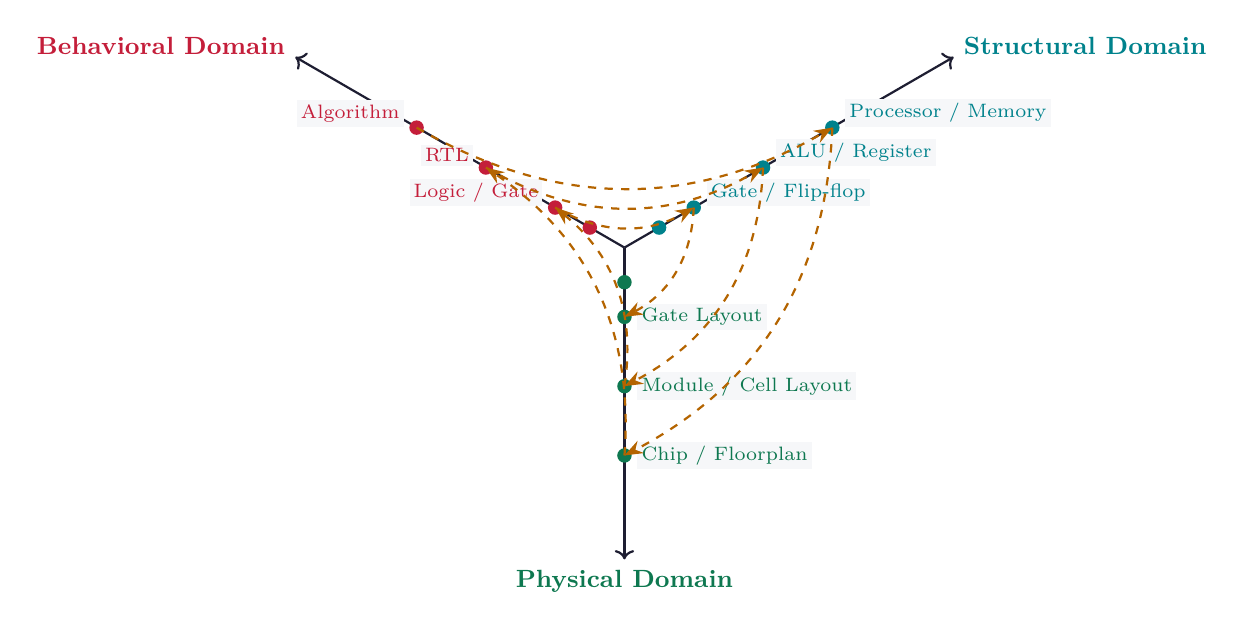
\begin{tikzpicture}[scale=1.1, thick, font=\small]
  % Draw three axes radiating from center (extended to prevent text collision)
  \draw[line, ->] (0, 0) -- (-3.8, 2.2) node[above left, color=myred, yshift=-0.1cm] {\textbf{Behavioral Domain}};
  \draw[line, ->] (0, 0) -- (3.8, 2.2) node[above right, color=myteal, yshift=-0.1cm] {\textbf{Structural Domain}};
  \draw[line, ->] (0, 0) -- (0, -3.6) node[below, color=mygreen] {\textbf{Physical Domain}};

  % Abstraction levels markers (Behavioral) - shifted and styled with background fill to prevent curve collision
  \filldraw[myred] (-2.4, 1.385) circle (2pt) node[above left, font=\scriptsize, fill=mygray, inner sep=1.5pt, xshift=-0.15cm] {Algorithm};
  \filldraw[myred] (-1.6, 0.924) circle (2pt) node[above left, font=\scriptsize, fill=mygray, inner sep=1.5pt, xshift=-0.15cm] {RTL};
  \filldraw[myred] (-0.8, 0.462) circle (2pt) node[above left, font=\scriptsize, fill=mygray, inner sep=1.5pt, xshift=-0.15cm] {Logic / Gate};
  \filldraw[myred] (-0.4, 0.231) circle (2pt);

  % Abstraction levels markers (Structural) - shifted and styled with background fill to prevent curve collision
  \filldraw[myteal] (2.4, 1.385) circle (2pt) node[above right, font=\scriptsize, fill=mygray, inner sep=1.5pt, xshift=0.15cm] {Processor / Memory};
  \filldraw[myteal] (1.6, 0.924) circle (2pt) node[above right, font=\scriptsize, fill=mygray, inner sep=1.5pt, xshift=0.15cm] {ALU / Register};
  \filldraw[myteal] (0.8, 0.462) circle (2pt) node[above right, font=\scriptsize, fill=mygray, inner sep=1.5pt, xshift=0.15cm] {Gate / Flip-flop};
  \filldraw[myteal] (0.4, 0.231) circle (2pt);

  % Abstraction levels markers (Physical) - shifted and styled with background fill to prevent curve collision
  \filldraw[mygreen] (0, -2.4) circle (2pt) node[right, font=\scriptsize, fill=mygray, inner sep=1.5pt, xshift=0.15cm] {Chip / Floorplan};
  \filldraw[mygreen] (0, -1.6) circle (2pt) node[right, font=\scriptsize, fill=mygray, inner sep=1.5pt, xshift=0.15cm] {Module / Cell Layout};
  \filldraw[mygreen] (0, -0.8) circle (2pt) node[right, font=\scriptsize, fill=mygray, inner sep=1.5pt, xshift=0.15cm] {Gate Layout};
  \filldraw[mygreen] (0, -0.4) circle (2pt);

  % Draw synthesis spirals/arrows showing mapping from behavioral to structural to physical
  \draw[arrow, color=myamber, bend right=30, dashed] (-2.4, 1.385) to (2.4, 1.385);
  \draw[arrow, color=myamber, bend left=30, dashed] (2.4, 1.385) to (0, -2.4);
  
  \draw[arrow, color=myamber, bend right=30, dashed] (0, -2.4) to (-1.6, 0.924);
  \draw[arrow, color=myamber, bend right=30, dashed] (-1.6, 0.924) to (1.6, 0.924);
  \draw[arrow, color=myamber, bend left=30, dashed] (1.6, 0.924) to (0, -1.6);
  
  \draw[arrow, color=myamber, bend right=30, dashed] (0, -1.6) to (-0.8, 0.462);
  \draw[arrow, color=myamber, bend right=30, dashed] (-0.8, 0.462) to (0.8, 0.462);
  \draw[arrow, color=myamber, bend left=30, dashed] (0.8, 0.462) to (0, -0.8);
\end{tikzpicture}
\end{tcolorbox}

\subsection{Design Hierarchy (Top-Down vs. Bottom-Up)}
\begin{itemize}[leftmargin=*, itemsep=3.5pt]
  \item \textbf{Top-Down Design Flow}: Starts at the system level (behavioral description) and recursively decomposes the system into functional blocks down to logic gates and transistor layouts. Highly automated and preferred for complex VLSI chips.
  \item \textbf{Bottom-Up Design Flow}: Starts at the lowest transistor level, building basic library cells (NAND, Flip-Flops) and grouping them into larger blocks until the system-level chip is constructed. Used for custom analog blocks and layout optimizations.
\end{itemize}

\section{VLSI Design Styles}

\subsection{Full Custom Design}
Every transistor, wire, and layer is custom-designed manually.
\begin{itemize}[leftmargin=*, itemsep=3.5pt]
  \item \textbf{Features}: Yields the highest possible performance, smallest silicon area, and lowest power dissipation.
  \item \textbf{Drawbacks}: Extremely high engineering cost, very long design cycle (time-to-market), and high risk of errors. Reserved for high-volume processors and analog blocks.
\end{itemize}

\subsection{Semi-Custom Design}
\begin{itemize}[leftmargin=*, itemsep=3.5pt]
  \item \textbf{Standard-Cell Based Design:} Layout is composed of pre-designed, pre-tested cell libraries (AND, flip-flops) placed in rows. Wires are routed automatically in channels between cell rows. Offers a balance between performance, design time, and cost.
  \item \textbf{Gate Array Based Design:} Wafers containing regular arrays of uncommitted transistors are pre-fabricated up to the metal contact level. Design customization is done only on the final metal interconnect mask layers. Very fast turnaround time and low mask cost, but lower utilization and speed.
  \item \textbf{FPGA (Field Programmable Gate Array):} Contains pre-fabricated programmable logic blocks (LUTs) and routing matrices. Configured electrically by loading configuration bits (RAM/Flash) without mask fabrication. Zero mask cost, instant turnaround, but has higher area and lower speed compared to ASICs.
\end{itemize}

\begin{tcolorbox}[tikzbox, title={Comparison of Design Methodologies}]
\renewcommand{\arraystretch}{1.4}
\par\noindent
\begin{tabularx}{\linewidth}{|B{2.2cm}|Y|Y|Y|}
\hline
\textbf{Feature} & \textbf{\color{myred}Full Custom} & \textbf{\color{myteal}Standard-Cell} & \textbf{\color{myamber}FPGA} \\
\hline
\textbf{Design Time} & Very Long (Months/Years) & Medium (Weeks/Months) & Very Short (Hours/Days) \\
\hline
\textbf{NRE Mask Cost} & Extremely High & High & Zero \\
\hline
\textbf{Performance} & Maximum & High & Moderate \\
\hline
\textbf{Unit Cost} & Low (at high volume) & Medium & High (due to overhead) \\
\hline
\textbf{Flexibility} & Zero (after tape-out) & Zero (after tape-out) & Re-programmable \\
\hline
\end{tabularx}
\end{tcolorbox}

\newpage
% ===============================================================================
\section{MOSFET Physical Operation}
% ===============================================================================

An n-channel MOSFET consists of a p-type silicon substrate (body), two heavily doped n+ regions (source and drain), and a metal/polysilicon gate insulated from the substrate by a thin silicon dioxide ($\text{SiO}_2$) layer.

\subsection{MOS Capacitor Operating Regions}
With the source and body grounded ($V_S = V_B = 0\,\text{V}$), as the gate voltage $V_G$ increases:
\begin{enumerate}[label=\alph*., leftmargin=*]
  \item \textbf{Accumulation ($V_G < V_{FB}$):} Negative charge on the gate attracts majority holes from the p-substrate to the silicon-oxide interface.
  \item \textbf{Depletion ($V_{FB} < V_G < V_{th}$):} Small positive gate voltage repels holes away from the interface, leaving behind fixed, negative acceptor ions ($N_A^-$), forming a carrier-free depletion region.
  \item \textbf{Inversion ($V_G > V_{th}$):} A large positive gate voltage bends the energy bands down sufficiently to attract minority electrons from the substrate and n+ source/drain to the interface. This forms a thin, conducting n-channel directly beneath the oxide.
\end{enumerate}

\subsection{Threshold Voltage ($V_{th}$)}
The threshold voltage is the minimum gate-to-source voltage required to induce strong inversion (creation of the conducting channel).

\begin{tcolorbox}[formulabox, title={\textbf{Threshold Voltage Formula}}]
For a p-substrate device:
\begin{equation}
  V_{th} = \Phi_{MS} + 2\phi_F - \frac{Q_{ox}}{C_{ox}} - \frac{Q_d}{C_{ox}}
\end{equation}
where:
\begin{itemize}[leftmargin=*, itemsep=2pt, topsep=2pt]
  \item $\Phi_{MS}$: Metal-semiconductor work function difference.
  \item $\phi_F$: Bulk Fermi potential: $\phi_F = V_T \ln(N_A / n_i)$.
  \item $Q_{ox}$: Fixed oxide interface charge.
  \item $Q_d$: Depletion region charge: $Q_d = -\sqrt{2q\epsilon_{si}N_A(2\phi_F + V_{SB})}$.
  \item $C_{ox}$: Gate oxide capacitance per unit area: $C_{ox} = \epsilon_{ox}/t_{ox}$.
\end{itemize}
\end{tcolorbox}

\subsection{Body Effect}
When the source-to-body junction is reverse-biased ($V_{SB} > 0$), the depletion region thickness increases, exposing more negative acceptor ions. The gate must support this extra depletion charge before inversion can occur, increasing the threshold voltage.

\begin{tcolorbox}[formulabox, title={\textbf{Body Effect Expression}}]
The shifted threshold voltage is expressed as:
\begin{equation}
  V_{th} = V_{th0} + \gamma \left( \sqrt{|2\phi_F| + V_{SB}} - \sqrt{|2\phi_F|} \right)
\end{equation}
where:
\begin{itemize}[leftmargin=*, itemsep=2pt, topsep=2pt]
  \item $V_{th0}$: Threshold voltage at zero body bias ($V_{SB} = 0$).
  \item $\gamma$: Body effect coefficient: $\gamma = \frac{\sqrt{2q\epsilon_{si}N_A}}{C_{ox}}$ (units: $\text{V}^{1/2}$).
  \item $V_{SB}$: Source-to-body reverse bias voltage.
\end{itemize}
\end{tcolorbox}

\subsection{Channel Length Modulation (CLM)}
In saturation ($V_{DS} > V_{GS} - V_{th}$), the channel pinches off at the drain end. Further increases in $V_{DS}$ cause the pinch-off point to move toward the source, reducing the effective channel length to $L_{eff} = L - \Delta L$.
\textbf{Effect}: Because current is inversely proportional to channel length ($I_D \propto 1/L_{eff}$), the channel shortening causes the drain current to rise with $V_{DS}$ rather than saturating completely:
  \begin{equation}
    I_{D,\text{sat}} \propto \left( 1 + \lambda V_{DS} \right)
  \end{equation}
  where $\lambda$ is the channel length modulation parameter ($\text{V}^{-1}$).

\subsection{Short-Channel Effects (SCE)}
Short-channel effects occur when the physical channel length $L$ is of the same order of magnitude as the source/drain depletion region widths.
\begin{itemize}[leftmargin=*, itemsep=3.5pt]
  \item \textbf{Drain-Induced Barrier Lowering (DIBL):} High drain voltage lowers the source-channel potential barrier, allowing extra electrons to inject into the channel, reducing $V_{th}$ and increasing subthreshold leakage.
  \item \textbf{Charge Sharing:} The gate depletion region overlaps with the source/drain depletion regions. Part of the depletion charge is supported by the source/drain junctions rather than the gate, lowering the gate charge required for inversion $\implies V_{th}$ decreases.
  \item \textbf{Velocity Saturation:} In short channels, the longitudinal electric field ($E = V_{DS}/L$) is very high. Carrier drift velocity saturates ($v_{\text{sat}} \approx 10^7\,\text{cm/s}$) due to phonon scattering, making the drain current linear with $V_{GS}$ instead of quadratic.
  \item \textbf{Hot Carrier Injection (HCI):} High-energy electrons near the drain generate electron-hole pairs via impact ionization. Some electrons gain enough energy to penetrate the gate oxide, creating interface states that drift $V_{th}$ over time.
\end{itemize}

\newpage
% ===============================================================================
% MANDATORY QUICK REVISION PAGE
% ===============================================================================
\begin{center}
  {\large\bfseries\color{myred} Quick Revision --- Module 1}\\[3pt]
  {\small\color{mydark} VLSI Design Flow \& MOSFET Physics $|$ PE-EC603C}
\end{center}
\noindent{\color{myred}\rule{\linewidth}{1.2pt}}
\vspace{4pt}

\begin{tcolorbox}[formulabox, title={\textbf{Key Module 1 Formulas}}]
$$\text{Threshold Voltage:} \quad V_{th} = V_{th0} + \gamma \left( \sqrt{|2\phi_F| + V_{SB}} - \sqrt{|2\phi_F|} \right)$$
$$\text{Body Effect Coefficient:} \quad \gamma = \frac{\sqrt{2q\epsilon_{si}N_A}}{C_{ox}} \qquad \text{Bulk Potential:} \quad \phi_F = V_T \ln\left(\frac{N_A}{n_i}\right)$$
$$\text{Oxide Capacitance:} \quad C_{ox} = \frac{\epsilon_{ox}}{t_{ox}} \qquad \text{CLM Saturation factor:} \quad (1 + \lambda V_{DS})$$
\end{tcolorbox}

\begin{tcolorbox}[defbox, title={\textbf{One-Line Definitions}}]
\begin{itemize}[leftmargin=*, itemsep=2.5pt, topsep=0pt]
  \item \textbf{Moore's Law:} Observation stating that transistor density doubles every 2 years while cost drops.
  \item \textbf{Y-Chart:} Visual model categorizing VLSI design along behavioral, structural, and physical domains.
  \item \textbf{Strong Inversion:} State where gate voltage is high enough to make channel electron concentration equal to bulk hole doping.
  \item \textbf{Body Effect:} Increase in threshold voltage due to negative source-to-body substrate bias.
  \item \textbf{Channel Length Modulation:} Pinch-off point migration under high drain bias, shortening effective channel length.
  \item \textbf{DIBL:} Short-channel threshold drop caused by the drain potential lowering the source junction injection barrier.
  \item \textbf{Velocity Saturation:} Saturation of carrier drift velocity under high electric fields in short channels.
\end{itemize}
\end{tcolorbox}

\begin{tcolorbox}[exambox, title={\textbf{Frequently Asked / Viva Questions}}]
\begin{enumerate}[topsep=0pt, label=\textbf{Q\arabic*.}, itemsep=5pt]
  \item \Q{What is the Gajski-Yuhan Y-Chart and how is it used in VLSI?}
    The Y-chart defines the design abstraction levels (System, RTL, Logic, Circuit) along three domains: Behavioral, Structural, and Physical. The design flow is a spiral mapping that translates behavioral specifications into structural connections, which are then placed and routed into physical layout masks.
  \item \Q{Compare Gate Array and Standard-Cell based design styles.}
    Standard-cell design uses fully customized layers and pre-designed logic libraries, offering high density and performance but higher mask costs. Gate arrays use pre-fabricated transistors up to the metal contact layer, customizing only interconnect masks, which reduces mask costs and manufacturing time but lowers speed.
  \item \Q{Why does the threshold voltage increase with reverse body bias ($V_{SB} > 0$)?}
    Reverse biasing the source-body junction widens the depletion layer beneath the gate, exposing more ionized acceptor impurities ($N_A^-$). The gate voltage must support this additional depletion charge before it can create the inversion channel, raising the required threshold voltage.
  \item \Q{What is flat-band voltage and flat-band condition?}
    Flat-band voltage ($V_{FB}$) is the gate voltage at which there is no charge on the gate and no net charge in the silicon substrate. Under this condition, the energy bands in the semiconductor remain perfectly flat up to the oxide interface.
  \item \Q{Explain the physical cause of Channel Length Modulation (CLM).}
    When the drain voltage $V_{DS}$ exceeds the overdrive voltage ($V_{GS} - V_{th}$), the channel pinch-off point moves away from the drain. The voltage drop across the remaining inverted channel remains locked at $V_{DS,\text{sat}} = V_{GS} - V_{th}$, while the excess voltage ($V_{DS} - V_{DS,\text{sat}}$) is dropped across the depletion region near the drain, physically shortening the channel.
  \item \Q{What is Drain-Induced Barrier Lowering (DIBL) and how does it affect $V_{th}$?}
    In short-channel devices, the drain depletion region extends deep into the channel. When high drain voltage is applied, its electric field lines penetrate under the gate oxide, lowering the potential barrier between the source and the channel. This allows subthreshold conduction to begin at a lower gate voltage, lowering $V_{th}$.
  \item \Q{What is velocity saturation and what is its effect on the saturation current of a short-channel MOSFET?}
    At high electric fields ($E \approx 10^4\,\text{V/cm}$), carrier velocity saturates due to collision scattering. In a short-channel MOSFET, this causes the drain current to become linearly proportional to $V_{GS}$ ($I_{D,\text{sat}} \propto V_{GS} - V_{th}$) instead of quadratic, limiting the speed/drive current.
  \item \Q{Describe Hot Carrier Injection (HCI).}
    HCI occurs when carriers gain high kinetic energy from the large electric field near the drain. These "hot" carriers undergo impact ionization, and some gain enough energy to jump over the $\text{SiO}_2$ barrier into the gate oxide, trapping charge. This leads to threshold voltage shifts and device degradation over time.
  \item \Q{Why is FPGA design preferred for low-volume applications?}
    Because FPGAs do not require custom silicon mask fabrication, eliminating non-recurring engineering (NRE) costs. The hardware can be re-programmed instantly, making it highly cost-effective and faster for low-volume designs.
  \item \Q{Define the terms: Accumulation, Depletion, and Inversion in an MOS capacitor.}
    Accumulation is the drawing of majority holes to the interface when $V_G < 0$. Depletion is the pushing away of holes, leaving a depletion charge when $V_G > 0$ but below $V_{th}$. Inversion is the drawing of minority electrons to create a conducting channel when $V_G > V_{th}$.
\end{enumerate}
\end{tcolorbox}


% -- Module 2 -----------------------------------------------------------------
\modulestart{2}{MOSFET Current Expression Derivation}

\section{MOSFET Current Expression Derivation}
% ===============================================================================

To derive the current-voltage ($I_D-V_{DS}$) characteristics of a MOSFET, we utilize the \textbf{Gradual Channel Approximation (GCA)}.

\begin{tcolorbox}[defbox, title={\textbf{Gradual Channel Approximation (GCA)}}]
GCA assumes that the electric field perpendicular to the channel (transverse field $E_x$ created by gate voltage) is much larger than the electric field parallel to the channel (longitudinal field $E_y$ created by drain-to-source voltage): $|E_x| \gg |E_y| \implies \left|\frac{\partial E_x}{\partial x}\right| \gg \left|\frac{\partial E_y}{\partial y}\right|$.
\end{tcolorbox}

\begin{tcolorbox}[tikzbox, title={n-channel MOSFET Cross-Section}]
\centering
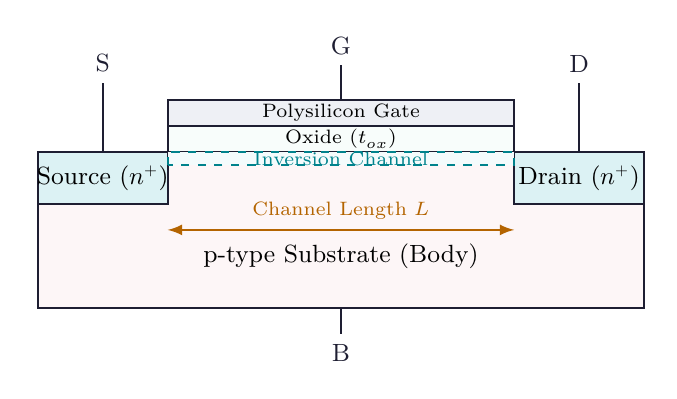
\begin{tikzpicture}[scale=1.1, thick, font=\small]
  % Substrate (P-type)
  \draw[draw=mydark, fill=hdrred!40] (-3.5, -1.8) rectangle (3.5, 0);
  \node at (0, -1.2) {p-type Substrate (Body)};
  
  % Source and Drain (N+ regions)
  \draw[draw=mydark, fill=hdrteal] (-3.5, -0.6) rectangle (-2.0, 0);
  \node at (-2.75, -0.3) {Source ($n^+$)};
  \draw[draw=mydark, fill=hdrteal] (2.0, -0.6) rectangle (3.5, 0);
  \node at (2.75, -0.3) {Drain ($n^+$)};
  
  % Gate Oxide
  \draw[draw=mydark, fill=hdrgreen!20] (-2.0, 0) rectangle (2.0, 0.3);
  \node[font=\scriptsize] at (0, 0.15) {Oxide ($t_{ox}$)};
  
  % Gate electrode
  \draw[draw=mydark, fill=hdrgray] (-2.0, 0.3) rectangle (2.0, 0.6);
  \node[font=\scriptsize] at (0, 0.45) {Polysilicon Gate};
  
  % Inversion channel
  \draw[draw=myteal, fill=hdrteal!30, dashed] (-2.0, -0.15) rectangle (2.0, 0);
  \node[font=\scriptsize, color=myteal] at (0, -0.08) {Inversion Channel};
  
  % Terminals and contacts
  \draw[line] (-2.75, 0) -- (-2.75, 0.8) node[above] {S};
  \draw[line] (0, 0.6) -- (0, 1.0) node[above] {G};
  \draw[line] (2.75, 0) -- (2.75, 0.8) node[above] {D};
  \draw[line] (0, -1.8) -- (0, -2.1) node[below] {B};
  
  % Dimension indicators
  \draw[latex-latex, color=myamber] (-2.0, -0.9) -- node[above, font=\scriptsize] {Channel Length $L$} (2.0, -0.9);
\end{tikzpicture}
\end{tcolorbox}

\subsection{Linear Region Derivation}
Let the coordinate along the channel be $y$, where $y = 0$ at the source and $y = L$ at the drain. Let $V(y)$ be the channel potential at position $y$.
The local mobile inversion charge density per unit area $Q_I(y)$ is:
\begin{equation}
  Q_I(y) = -C_{ox} \left[ V_{GS} - V(y) - V_{th} \right]
\end{equation}
The drift current in the channel is driven by the longitudinal electric field $E_y = -dV(y)/dy$. The drain current $I_D$ at any point $y$ is:
\begin{equation}
  I_D = W \cdot Q_I(y) \cdot v_y(y)
\end{equation}
where $W$ is the channel width, and $v_y(y)$ is the drift velocity of electrons: $v_y(y) = -\mu_n E_y(y) = \mu_n \frac{dV(y)}{dy}$.
Substituting the expressions:
\begin{equation}
  I_D = W \cdot \left( -C_{ox} \left[ V_{GS} - V(y) - V_{th} \right] \right) \cdot \left( -\mu_n \frac{dV(y)}{dy} \right)
\end{equation}
\begin{equation}
  I_D = \mu_n C_{ox} W \left[ V_{GS} - V(y) - V_{th} \right] \frac{dV(y)}{dy}
\end{equation}
Rearranging terms:
\begin{equation}
  I_D \cdot dy = \mu_n C_{ox} W \left[ V_{GS} - V_{th} - V(y) \right] dV(y)
\end{equation}
Integrating along the channel length from the source ($y=0, V(0)=0$) to the drain ($y=L, V(L)=V_{DS}$):
\begin{equation}
  \int_{0}^{L} I_D \, dy = \mu_n C_{ox} W \int_{0}^{V_{DS}} \left[ V_{GS} - V_{th} - V \right] dV
\end{equation}
Since $I_D$ is constant throughout the channel:
\begin{equation}
  I_D \cdot L = \mu_n C_{ox} W \left[ (V_{GS} - V_{th})V - \frac{V^2}{2} \right]_{0}^{V_{DS}}
\end{equation}
\begin{equation}
  I_D = \mu_n C_{ox} \frac{W}{L} \left[ (V_{GS} - V_{th})V_{DS} - \frac{V_{DS}^2}{2} \right]
\end{equation}
This is the \textbf{MOSFET Linear Region Current Equation} (valid for $V_{DS} < V_{GS} - V_{th}$).

\subsection{Saturation Region Derivation}
As $V_{DS}$ increases, the channel charge density at the drain end drops to zero when $V_{DS} = V_{GS} - V_{th}$. This condition is called \textbf{pinch-off}.
The saturation current $I_{D,\text{sat}}$ remains constant with further increases in $V_{DS}$. Substituting the pinch-off voltage $V_{DS} = V_{GS} - V_{th}$ into the linear current equation:
\begin{equation}
  I_{D,\text{sat}} = \mu_n C_{ox} \frac{W}{L} \left[ (V_{GS} - V_{th})(V_{GS} - V_{th}) - \frac{(V_{GS} - V_{th})^2}{2} \right]
\end{equation}
\begin{equation}
  I_{D,\text{sat}} = \frac{1}{2} \mu_n C_{ox} \frac{W}{L} \left( V_{GS} - V_{th} \right)^2
\end{equation}
This is the \textbf{MOSFET Saturation Region Current Equation} (valid for $V_{DS} \ge V_{GS} - V_{th}$).

\section{MOSFET Scaling Principles}

Scaling refers to reducing the physical dimensions of the MOSFET (channel length $L$, width $W$, gate oxide thickness $t_{ox}$) by a factor of $\beta > 1$ to increase packing density and speed.

\subsection{Types of Scaling}
\begin{itemize}[leftmargin=*, itemsep=3.5pt]
  \item \textbf{Constant-Field Scaling (Full Scaling):} All physical dimensions ($W, L, t_{ox}$) and voltages ($V_{DD}, V_{th}$) are scaled down by the factor $1/\beta$. This keeps the internal electric fields constant, preventing breakdown.
  \item \textbf{Constant-Voltage Scaling:} Only physical dimensions are scaled down by $1/\beta$, while the supply voltage $V_{DD}$ remains unchanged. This preserves system compatibility with older circuits (e.g. 5V logic) but leads to very high electric fields inside the chip.
\end{itemize}

\subsection{Scaling Factors Summary}
The table below summarizes how physical parameters scale under both scaling paradigms:

\begin{tcolorbox}[tikzbox, title={Comparison of Scaling Paradigms}]
{\renewcommand{\arraystretch}{1.55}%
\par\noindent
\begin{tabularx}{\linewidth}{|B{3.2cm}|>{\small\centering\arraybackslash}X|>{\small\centering\arraybackslash}X|}
\hline
\textbf{Parameter} & \textbf{\color{myred}Constant-Field} & \textbf{\color{myteal}Constant-Voltage} \\
\hline
\textbf{Dimensions ($W, L, t_{ox}$)} & $1/\beta$ & $1/\beta$ \\
\hline
\textbf{Voltages ($V_{DD}, V_{th}$)} & $1/\beta$ & $1$ \\
\hline
\textbf{Electric Field ($E$)} & $1$ & $\beta$ \\
\hline
\textbf{Capacitance ($C_{ox}$)} & $\beta$ & $\beta$ \\
\hline
\textbf{Drain Current ($I_D$)} & $1/\beta$ & $\beta$ \\
\hline
\textbf{Gate Delay ($\tau$)} & $1/\beta$ & $1/\beta^2$ \\
\hline
\textbf{Power Dissipation ($P$)} & $1/\beta^2$ & $\beta$ \\
\hline
\textbf{Power Density ($P/\text{Area}$)} & $1$ & $\beta^3$ \\
\hline
\end{tabularx}}
\end{tcolorbox}

\begin{tcolorbox}[examplebox, title={\textbf{Warning: Power Density Escalation}}]
Under Constant-Voltage scaling, the power density increases by $\beta^3$. This causes massive heat dissipation issues in sub-micron chips, making Constant-Field (or hybrid) scaling mandatory for modern deep sub-micron VLSI designs.
\end{tcolorbox}

\newpage
% ===============================================================================
% MANDATORY QUICK REVISION PAGE
% ===============================================================================
\begin{center}
  {\large\bfseries\color{myred} Quick Revision --- Module 2}\\[3pt]
  {\small\color{mydark} MOSFET Current Derivation \& Scaling $|$ PE-EC603C}
\end{center}
\noindent{\color{myred}\rule{\linewidth}{1.2pt}}
\vspace{4pt}

\begin{tcolorbox}[formulabox, title={\textbf{Key Module 2 Formulas}}]
$$\text{Linear Current:} \quad I_D = \mu_n C_{ox} \frac{W}{L} \left[ (V_{GS} - V_{th})V_{DS} - \frac{V_{DS}^2}{2} \right]$$
$$\text{Saturation Current:} \quad I_{D,\text{sat}} = \frac{1}{2} \mu_n C_{ox} \frac{W}{L} (V_{GS} - V_{th})^2 \left( 1 + \lambda V_{DS} \right)$$
$$\text{Pinch-off Condition:} \quad V_{DS,\text{sat}} = V_{GS} - V_{th} \qquad C_{ox} = \frac{\epsilon_{ox}}{t_{ox}}$$
\end{tcolorbox}

\begin{tcolorbox}[defbox, title={\textbf{One-Line Definitions}}]
\begin{itemize}[leftmargin=*, itemsep=2.5pt, topsep=0pt]
  \item \textbf{GCA:} Approximation assuming channel potential variations are much slower than gate oxide potential drops.
  \item \textbf{Pinch-off:} Condition where the inversion channel charge vanishes at the drain end ($V_{DS} = V_{GS} - V_{th}$).
  \item \textbf{Constant-Field Scaling:} Scaling method where dimensions and voltages are reduced by $\beta$ to keep internal fields constant.
  \item \textbf{Constant-Voltage Scaling:} Scaling method where dimensions are reduced by $\beta$ while voltages remain constant.
  \item \textbf{Subthreshold Current:} Leakage current that flows from drain to source even when $V_{GS} < V_{th}$.
  \item \textbf{Drift Velocity:} Average velocity attained by charged particles (electrons) in a material due to an electric field.
\end{itemize}
\end{tcolorbox}

\begin{tcolorbox}[exambox, title={\textbf{Frequently Asked / Viva Questions}}]
\begin{enumerate}[topsep=0pt, label=\textbf{Q\arabic*.}, itemsep=5pt]
  \item \Q{State the Gradual Channel Approximation (GCA) and its physical validity.}
    GCA assumes the longitudinal field along the channel $E_y = dV/dy$ changes very slowly compared to the vertical field $E_x$ across the oxide. It is highly valid for long-channel devices ($L \gg t_{ox}$), but breaks down in short-channel devices where $E_y$ is extremely high.
  \item \Q{Derive the drain current equation for a MOSFET operating in the linear region.}
    Starting with charge density $Q_I(y) = -C_{ox}(V_{GS} - V(y) - V_{th})$ and current $I_D = W Q_I(y) \mu_n (dV/dy)$, we integrate from $y=0$ to $L$ and $V=0$ to $V_{DS}$ to obtain the linear equation: $I_D = \mu_n C_{ox} \frac{W}{L} [(V_{GS} - V_{th})V_{DS} - V_{DS}^2 / 2]$.
  \item \Q{Explain the concept of channel pinch-off.}
    Pinch-off occurs when the voltage difference between the gate and the channel at the drain end falls below the threshold voltage, i.e., $V_{GD} = V_{GS} - V_{DS} = V_{th}$. At this point, the local inversion charge density at the drain becomes zero, and the current saturates.
  \item \Q{Why does Constant-Voltage scaling lead to reliability issues in sub-micron devices?}
    Because the physical dimensions ($L, t_{ox}$) are scaled down by $1/\beta$ while supply voltage stays constant, the internal electric fields increase by a factor of $\beta$. This causes oxide breakdown, hot-carrier injection, and velocity saturation.
  \item \Q{A MOSFET has $W = 10\,\mu\text{m}$, $L = 1\,\mu\text{m}$, $\mu_n C_{ox} = 100\,\mu\text{A/V}^2$, and $V_{th} = 0.8\,\text{V}$. Find $I_D$ at $V_{GS} = 2.0\,\text{V}$ and $V_{DS} = 0.5\,\text{V}$.}\\
    Here $V_{GS} - V_{th} = 2.0 - 0.8 = 1.2\,\text{V}$. Since $V_{DS} = 0.5\,\text{V} < 1.2\,\text{V}$, the device is in the linear region.\par
    $I_D = 100 \times 10 \left[ (1.2)(0.5) - 0.25/2 \right] = 1000 \left[ 0.6 - 0.125 \right] = 475\,\mu\text{A}$.
  \item \Q{Calculate the saturation current $I_{D,\text{sat}}$ for the same device ($V_{GS} = 2.0\,\text{V}, V_{DS} = 1.5\,\text{V}$).}\\
    Since $V_{DS} = 1.5\,\text{V} > 1.2\,\text{V}$, the device is in saturation.\par
    $I_{D,\text{sat}} = \frac{1}{2} \mu_n C_{ox} \frac{W}{L} (V_{GS} - V_{th})^2 = \frac{1}{2} \cdot 100 \cdot 10 \cdot (1.2)^2 = 500 \cdot 1.44 = 720\,\mu\text{A}$.
  \item \Q{Why does power density remain constant under constant-field scaling?}
    Under constant-field scaling, the power $P$ scales by $1/\beta^2$ and the chip area ($W \times L$) scales by $1/\beta^2$. Therefore, the ratio $P/\text{Area}$ scales by $(1/\beta^2)/(1/\beta^2) = 1$, keeping the thermal density constant.
  \item \Q{Derive the scaling factor of gate delay $\tau$ in constant-field scaling.}
    Gate delay is $\tau = \frac{C \cdot V}{I}$. Capacitance $C \propto W \cdot L / t_{ox}$ scales by $1/\beta$, voltage $V$ scales by $1/\beta$, and current $I$ scales by $1/\beta$. Thus, $\tau$ scales by $\frac{(1/\beta) \cdot (1/\beta)}{1/\beta} = 1/\beta$ (speed increases by $\beta$).
  \item \Q{What is the effect of channel length modulation on the saturation drain current?}
    It adds a term $(1 + \lambda V_{DS})$ to the saturation current equation. This represents the fact that after pinch-off, the effective channel length shortens as $V_{DS}$ increases, causing a small, linear increase in current rather than a flat saturation.
  \item \Q{Why is electron mobility ($\mu_n$) higher than hole mobility ($\mu_p$)?}
    Electrons reside in the conduction band where they have lower effective mass and experience less lattice scattering than holes, which move through the valence band by bond-breaking. This makes $\mu_n \approx 2.5$ to $3$ times higher than $\mu_p$.
\end{enumerate}
\end{tcolorbox}


% -- Module 3 -----------------------------------------------------------------
\modulestart{3}{Unit Fabrication Processes in VLSI}

\section{Unit Fabrication Processes in VLSI}
% ===============================================================================

IC fabrication involves a sequential series of chemical and physical processing steps performed on a high-purity silicon wafer substrate.

\subsection{Wafer Preparation}
Raw silicon dioxide (sand) is reduced to electronic-grade silicon (EGS). Wafers are cut from a single-crystal ingot grown via the \textbf{Czochralski (CZ) method}, followed by slicing, edge-rounding, grinding, and chemical-mechanical polishing (CMP) to create a defect-free surface.

\subsection{Oxidation}
The process of growing a thin layer of silicon dioxide ($\text{SiO}_2$) on the silicon surface. It is used as a gate oxide, masking layer, and passivation barrier.
\begin{itemize}[leftmargin=*, itemsep=3pt]
  \item \textbf{Dry Oxidation ($\text{Si} + \text{O}_2 \to \text{SiO}_2$):} Performed in pure oxygen gas. Growth is slow, but produces high-density, high-quality oxides. Used for thin gate oxides.
  \item \textbf{Wet Oxidation ($\text{Si} + 2\text{H}_2\text{O} \to \text{SiO}_2 + 2\text{H}_2$):} Performed in water vapor. Growth is very fast, but density is lower. Used for thick field oxides (FOX) or masking layers.
\end{itemize}

\begin{tcolorbox}[defbox, title={\textbf{Deal-Grove Model of Oxidation}}]
The oxide thickness $x_{ox}$ grown over time $t$ is expressed by the quadratic relation:
\begin{equation}
  x_{ox}^2 + A \cdot x_{ox} = B(t + \tau)
\end{equation}
\begin{itemize}[leftmargin=*, itemsep=2.5pt, topsep=2.5pt]
  \item \textbf{Short times (linear regime)}: $x_{ox} \approx \frac{B}{A}(t + \tau)$ (reaction rate-limited).
  \item \textbf{Long times (parabolic regime)}: $x_{ox} \approx \sqrt{B \cdot t}$ (diffusion-limited through existing oxide).
\end{itemize}
\end{tcolorbox}

\subsection{Photolithography}
A process used to transfer geometric patterns from a photo-mask onto the wafer surface.
1. \textbf{Coating}: Apply light-sensitive polymer liquid (\textbf{Photoresist - PR}) on the wafer and spin to distribute uniformly. Soft-bake to drive off solvents.
2. \textbf{Exposure}: Shine UV light through a chrome pattern photo-mask onto the PR layer.
   \begin{itemize}[leftmargin=*, noitemsep, topsep=2pt]
     \item \textbf{Positive PR}: Exposed regions become soluble in developer solution.
     \item \textbf{Negative PR}: Exposed regions polymerize/cross-link, becoming insoluble.
   \end{itemize}
3. \textbf{Development}: Wash away soluble photoresist in developer solution. Hard-bake to solidify the remaining PR pattern.

\subsection{Diffusion \& Ion Implantation}
These processes introduce dopant impurities (boron for p-type, phosphorus/arsenic for n-type) into selective regions of the silicon substrate:
\begin{itemize}[leftmargin=*, itemsep=3.5pt]
  \item \textbf{Diffusion}: High-temperature thermal process ($900^\circ\text{C}$--$1100^\circ\text{C}$). Dopant atoms diffuse isotropically (in all directions, leading to lateral junction spreading beneath the masks) following Fick's laws of diffusion.
  \item \textbf{Ion Implantation}: An energetic beam of dopant ions is accelerated in an electric field ($10$--$500\,\text{keV}$) and directed at the wafer. Ions penetrate vertically, creating a precise, anisotropic dopant profile. This causes lattice damage, requiring high-temperature \textbf{thermal annealing} to restore the crystal structure.
\end{itemize}

\subsection{Deposition (CVD \& PVD)}
Used to grow thin films of materials (polysilicon, silicon nitride, metals) on the wafer surface.
\begin{itemize}[leftmargin=*, itemsep=3pt]
  \item \textbf{Chemical Vapor Deposition (CVD):} Gaseous precursors react chemically at the wafer surface (e.g., thermal decomposition of silane to deposit polysilicon: $\text{SiH}_4 \to \text{Si} + 2\text{H}_2$).
  \item \textbf{Physical Vapor Deposition (PVD):} Physical transfer of atoms (sputtering or vacuum evaporation) from a metal target to the wafer. Used for metallization.
\end{itemize}

\subsection{Etching \& Chemical Mechanical Planarization (CMP)}
\begin{itemize}[leftmargin=*, itemsep=3.5pt]
  \item \textbf{Etching}: Selective removal of material not protected by photoresist.
  \begin{itemize}[leftmargin=*, noitemsep, topsep=2pt]
    \item \textbf{Wet Chemical Etching}: Isotropic, causes undercutting under the mask.
    \item \textbf{Reactive Ion Etching (RIE) / Dry Etching}: Anisotropic, uses gas plasma to etch vertically.
  \end{itemize}
  \item \textbf{CMP}: A chemical slurry and mechanical polishing pad process used to achieve flat, planar surfaces before subsequent lithography steps.
\end{itemize}

\section{CMOS Fabrication Process Flow}

CMOS circuits require the fabrication of both n-channel and p-channel MOSFETs on the same substrate. Since the substrate can only have one doping type (e.g., p-type), a localized well of the opposite type (e.g., n-well) must be created to house the complementary device.

\subsection{n-Well CMOS Process Flow Steps}
Starting with a p-type substrate:
1. \textbf{Well Formation}: Lithography and ion implantation of phosphorus/arsenic to create the \textbf{n-well region} (where pMOS transistors will be placed). Drive-in anneal.
2. \textbf{Active Area Definition}: Deposit silicon nitride ($\text{Si}_3\text{N}_4$) as a mask, pattern it, and grow thick \textbf{Field Oxide (FOX)} via local oxidation of silicon (LOCOS) to isolate active regions.
3. \textbf{Threshold Adjust Implants}: Implantation of boron to adjust the threshold voltages of both nMOS and pMOS devices.
4. \textbf{Gate Oxide Growth}: Grow high-quality, ultra-thin dry gate oxide layer ($\text{SiO}_2$).
5. \textbf{Polysilicon Gate Formation}: Deposit polysilicon via CVD, pattern it with lithography, and etch to form the gate electrodes.
6. \textbf{Source/Drain Implantation (Self-Aligned Gates)}:
   \begin{itemize}[leftmargin=*, noitemsep, topsep=2pt]
     \item Implant arsenic/phosphorus ($n^+$) to form nMOS source/drain and the n-well body contact tap. The polysilicon gate acts as a self-aligned mask for the channel.
     \item Implant boron ($p^+$) to form pMOS source/drain and the p-substrate body contact tap.
   \end{itemize}
7. \textbf{Interlevel Dielectric (ILD) Deposition}: Deposit thick insulating oxide layer, etch contact holes.
8. \textbf{Metallization}: Deposit metal (aluminum/copper) via PVD, pattern, and etch to form interconnects.

\begin{tcolorbox}[tikzbox, title={CMOS Inverter Fabrication Cross-Section}]
\centering
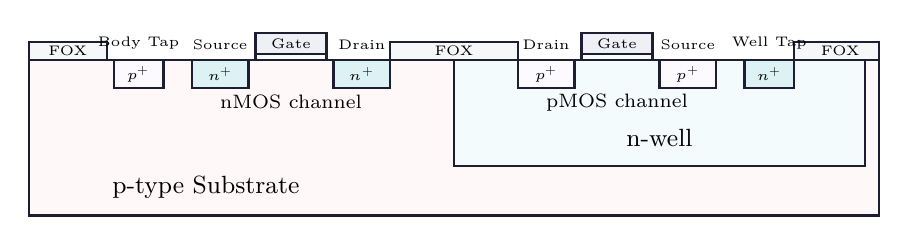
\begin{tikzpicture}[scale=0.9, thick, font=\small]
  % P-type Substrate
  \draw[draw=mydark, fill=hdrred!30] (-6.0, -2.2) rectangle (6.0, 0);
  \node at (-3.5, -1.8) {p-type Substrate};
  
  % N-well (on the right)
  \draw[draw=mydark, fill=hdrteal!30] (0.0, -1.5) rectangle (5.8, 0);
  \node at (2.9, -1.1) {n-well};
  
  % Field Oxide (FOX) Isolation blocks at surface
  \draw[draw=mydark, fill=mygray] (-6.0, 0) rectangle (-4.9, 0.25);
  \draw[draw=mydark, fill=mygray] (-0.9, 0) rectangle (0.9, 0.25);
  \draw[draw=mydark, fill=mygray] (4.8, 0) rectangle (6.0, 0.25);
  \node[font=\tiny] at (-5.45, 0.12) {FOX};
  \node[font=\tiny] at (0, 0.12) {FOX};
  \node[font=\tiny] at (5.45, 0.12) {FOX};
  
  % nMOS active implants (left)
  \draw[draw=mydark, fill=hdrpurple!20] (-4.8, -0.4) rectangle (-4.1, 0);
  \node[font=\tiny] at (-4.45, -0.2) {$p^+$};
  \draw[draw=mydark, fill=hdrteal] (-3.7, -0.4) rectangle (-2.9, 0);
  \node[font=\tiny] at (-3.3, -0.2) {$n^+$};
  \draw[draw=mydark, fill=hdrteal] (-1.7, -0.4) rectangle (-0.9, 0);
  \node[font=\tiny] at (-1.3, -0.2) {$n^+$};
  \node[font=\scriptsize] at (-2.3, -0.6) {nMOS channel};
  
  % pMOS active implants (right)
  \draw[draw=mydark, fill=hdrpurple!20] (0.9, -0.4) rectangle (1.7, 0);
  \node[font=\tiny] at (1.3, -0.2) {$p^+$};
  \draw[draw=mydark, fill=hdrpurple!20] (2.9, -0.4) rectangle (3.7, 0);
  \node[font=\tiny] at (3.3, -0.2) {$p^+$};
  \draw[draw=mydark, fill=hdrteal] (4.1, -0.4) rectangle (4.8, 0);
  \node[font=\tiny] at (4.45, -0.2) {$n^+$};
  \node[font=\scriptsize] at (2.3, -0.6) {pMOS channel};
  
  % Gate Oxides and Polysilicon Gates
  % nMOS Gate
  \draw[draw=mydark, fill=hdrgreen!20] (-2.8, 0) rectangle (-1.8, 0.08); % Oxide
  \draw[draw=mydark, fill=hdrgray] (-2.8, 0.08) rectangle (-1.8, 0.38); % Gate
  \node[font=\tiny] at (-2.3, 0.23) {Gate};
  
  % pMOS Gate
  \draw[draw=mydark, fill=hdrgreen!20] (1.8, 0) rectangle (2.8, 0.08); % Oxide
  \draw[draw=mydark, fill=hdrgray] (1.8, 0.08) rectangle (2.8, 0.38); % Gate
  \node[font=\tiny] at (2.3, 0.23) {Gate};

  % Text labels for implants
  \node[above, font=\tiny] at (-4.45, 0) {Body Tap};
  \node[above, font=\tiny] at (-3.3, 0) {Source};
  \node[above, font=\tiny] at (-1.3, 0) {Drain};
  \node[above, font=\tiny] at (1.3, 0) {Drain};
  \node[above, font=\tiny] at (3.3, 0) {Source};
  \node[above, font=\tiny] at (4.45, 0) {Well Tap};
\end{tikzpicture}
\end{tcolorbox}

\subsection{p-Well and Twin-Tub CMOS Processes}
\begin{itemize}[leftmargin=*, itemsep=3.5pt]
  \item \textbf{p-Well Process}: Starts with an n-type substrate. nMOS transistors are created inside a fabricated p-well, while pMOS transistors are fabricated directly in the n-substrate.
  \item \textbf{Twin-Tub Process}: Starts with a high-resistivity wafer containing an epitaxial layer. Both an n-well (tub) and a p-well (tub) are fabricated separately to optimize nMOS and pMOS channel profiles independently, eliminating threshold voltage offsets and minimizing latch-up risk.
\end{itemize}

\newpage
% ===============================================================================
% MANDATORY QUICK REVISION PAGE
% ===============================================================================
\begin{center}
  {\large\bfseries\color{myred} Quick Revision --- Module 3}\\[3pt]
  {\small\color{mydark} VLSI and IC Fabrication Technology $|$ PE-EC603C}
\end{center}
\noindent{\color{myred}\rule{\linewidth}{1.2pt}}
\vspace{4pt}

\begin{tcolorbox}[formulabox, title={\textbf{Key Fabrication Equations}}]
$$\text{Deal-Grove Model:} \quad x_{ox}^2 + A \cdot x_{ox} = B(t + \tau)$$
$$\text{Linear Oxide growth rate (thin):} \quad \frac{dx_{ox}}{dt} \approx \frac{B}{A} \qquad \text{Parabolic rate (thick):} \quad \frac{dx_{ox}}{dt} \approx \frac{B}{2x_{ox}}$$
$$\text{Fick's Second Law of Diffusion:} \quad \frac{\partial C(x,t)}{\partial t} = D \frac{\partial^2 C(x,t)}{\partial x^2}$$
\end{tcolorbox}

\begin{tcolorbox}[defbox, title={\textbf{One-Line Definitions}}]
\begin{itemize}[leftmargin=*, itemsep=2.5pt, topsep=0pt]
  \item \textbf{Czochralski Method:} Silicon crystal growth technique pulling single-crystal ingots from a liquid melt.
  \item \textbf{Dry Oxidation:} Oxidation utilizing pure oxygen gas, producing thin, highly uniform gate dielectric layers.
  \item \textbf{Wet Oxidation:} Oxidation utilizing steam water vapor, growing thick field oxides (FOX) rapidly.
  \item \textbf{Photoresist:} Light-sensitive organic polymer liquid used to transfer photomask geometric patterns.
  \item \textbf{Ion Implantation:} Anisotropic process accelerating dopant ions at high fields to target precise vertical depth profiles.
  \item \textbf{Self-Aligned Gate:} Technique where polysilicon gates act as masks for source/drain implants, preventing overlap offsets.
  \item \textbf{Twin-Tub CMOS:} Fabricating both n-well and p-well regions on epitaxial layers to optimize both transistor profiles.
\end{itemize}
\end{tcolorbox}

\begin{tcolorbox}[exambox, title={\textbf{Frequently Asked / Viva Questions}}]
\begin{enumerate}[topsep=0pt, label=\textbf{Q\arabic*.}, itemsep=5pt]
  \item \Q{Compare dry oxidation and wet oxidation in terms of growth rate, density, and application.}
    Dry oxidation uses pure oxygen; its growth rate is slow but it produces high-density, high-quality oxides, making it suitable for thin gate oxides. Wet oxidation uses steam; its growth rate is very fast but it yields lower density, making it suitable for thick field isolation oxides (FOX).
  \item \Q{Explain the difference between positive and negative photoresists.}
    In positive photoresists, exposure to UV light breaks down chemical bonds, making the exposed region highly soluble in the developer. In negative photoresists, UV exposure causes cross-linking, making the exposed region insoluble while unexposed regions wash away.
  \item \Q{Why is ion implantation preferred over thermal diffusion for doping?}
    Ion implantation is highly anisotropic, allowing precise independent control of both dose (total quantity of atoms) and depth (controlled by acceleration energy) with minimal lateral spreading under masks. Thermal diffusion is isotropic and spreads laterally.
  \item \Q{What is the Deal-Grove model and what are its two limiting regimes?}
    The Deal-Grove model describes the kinetics of thermal oxidation. The two limiting regimes are the linear regime (for thin oxides, reaction-rate limited at the silicon interface, $x_{ox} \propto t$) and the parabolic regime (for thick oxides, diffusion-limited through the existing $\text{SiO}_2$ layer, $x_{ox} \propto \sqrt{t}$).
  \item \Q{What is thermal annealing and why is it necessary after ion implantation?}
    During ion implantation, high-energy dopant ions bombard the silicon lattice, knocking atoms out of position and damaging the crystal structure. Thermal annealing heats the wafer (typically $900^\circ\text{C}$ to $1000^\circ\text{C}$) to repair the crystal lattice and electrically activate the dopants.
  \item \Q{Explain the term "Self-Aligned Gate" process.}
    In this process, the polysilicon gate is patterned first. During the subsequent source/drain ion implantation, the gate itself acts as a mask protecting the channel region. This guarantees perfect alignment of the source/drain junctions with the gate edges, eliminating overlap capacitances.
  \item \Q{What is the function of the body tap ($p^+$ in p-substrate) and well tap ($n^+$ in n-well)?}
    The body tap connects the p-substrate to the lowest potential (GND) and the well tap connects the n-well to the highest potential ($V_{DD}$). This keeps the parasitic p-substrate/n-well p-n junctions reverse-biased, preventing latch-up.
  \item \Q{What is Local Oxidation of Silicon (LOCOS) and what is its drawback?}
    LOCOS is a selective oxidation process using silicon nitride masks to grow thick field oxide (FOX) for isolating adjacent devices. Its drawback is the lateral diffusion of oxygen under the nitride mask, forming a sloped oxide region called the "bird's beak", which wastes active area.
  \item \Q{What is Shallow Trench Isolation (STI)?}
    STI is an isolation technique that replaces LOCOS in sub-micron technologies. It involves etching a shallow trench between active areas, filling it with deposited oxide (CVD), and planarizing it using CMP. It eliminates the bird's beak effect.
  \item \Q{Describe the Twin-Tub CMOS process and its benefits.}
    The Twin-Tub process creates both an n-well and a p-well tub inside a high-resistivity epitaxial layer. This allows the doping profiles, threshold voltages, and body effects of nMOS and pMOS transistors to be optimized independently.
\end{enumerate}
\end{tcolorbox}


% -- Module 4 -----------------------------------------------------------------
\modulestart{4}{CMOS Inverter Working \& Static Behavior}

\section{CMOS Inverter Working \& Static Behavior}
% ===============================================================================

The static CMOS inverter is the core combinational building block of digital VLSI circuits.

\subsection{Circuit Diagram and Operation}
It consists of a pull-up pMOS transistor (connected between $V_{DD}$ and $V_{out}$) and a pull-down nMOS transistor (connected between $V_{out}$ and GND).
\textbf{Operation}:
\begin{itemize}[leftmargin=*, itemsep=3.5pt]
  \item $V_{in} = 0\,\text{V}$ (Logic '0'): nMOS is cut-off; pMOS is ON (linear/saturated), pulling $V_{out}$ up to $V_{DD}$ (Logic '1').
  \item $V_{in} = V_{DD}$ (Logic '1'): pMOS is cut-off; nMOS is ON, pulling $V_{out}$ down to $0\,\text{V}$ (Logic '0').
\end{itemize}

\begin{tcolorbox}[tikzbox, title={CMOS Inverter Circuit \& Equivalent Switch Representation}]
\centering
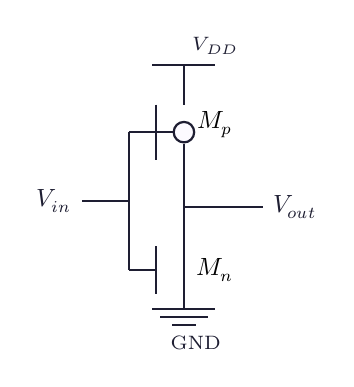
\begin{tikzpicture}[scale=1.0, thick, font=\small]
  % CMOS Schematic
  % pMOS
  \draw[line] (0, 1.8) -- (0, 1.3);
  \draw[draw=mydark, fill=hdrpurple!20] (0, 0.95) circle (0.13); % circle for pMOS gate
  \draw[line] (0, 0.8) -- (0, 0.3);
  \draw[line] (-0.7, 0.95) -- (-0.13, 0.95);
  \draw[line] (-0.35, 1.3) -- (-0.35, 0.6);
  \draw[line] (-0.35, 0.95) -- (-0.7, 0.95);
  \node at (0.4, 1.05) {$M_p$};

  % nMOS
  \draw[line] (0, -0.3) -- (0, -0.8);
  \draw[line] (0, -0.8) -- (0, -1.3);
  \draw[line] (-0.7, -0.8) -- (-0.35, -0.8);
  \draw[line] (-0.35, -0.5) -- (-0.35, -1.1);
  \node at (0.4, -0.8) {$M_n$};

  % Connections
  \draw[line] (-0.7, 0.95) -- (-0.7, -0.8);
  \draw[line] (-0.7, 0.075) -- (-1.3, 0.075) node[left] {$V_{in}$};
  \draw[line] (0, 0.3) -- (0, -0.3);
  \draw[line] (0, 0) -- (1.0, 0) node[right] {$V_{out}$};

  % Power Rails
  \draw[line] (-0.4, 1.8) -- (0.4, 1.8) node[above, font=\scriptsize] {$V_{DD}$};
  \draw[line] (-0.4, -1.3) -- (0.4, -1.3);
  \draw[line] (-0.3, -1.4) -- (0.3, -1.4);
  \draw[line] (-0.15, -1.5) -- (0.15, -1.5) node[below, font=\scriptsize] {GND};
\end{tikzpicture}
\end{tcolorbox}

\section{Voltage Transfer Characteristics (VTC)}

The VTC plot of $V_{out}$ vs. $V_{in}$ characterizes the inverter's static response.

\subsection{Five Regions of Operation}
The VTC curve is divided into 5 distinct regions based on the state of the two transistors:

\begin{tcolorbox}[tikzbox, title={CMOS Inverter Voltage Transfer Characteristics (VTC)}]
\centering
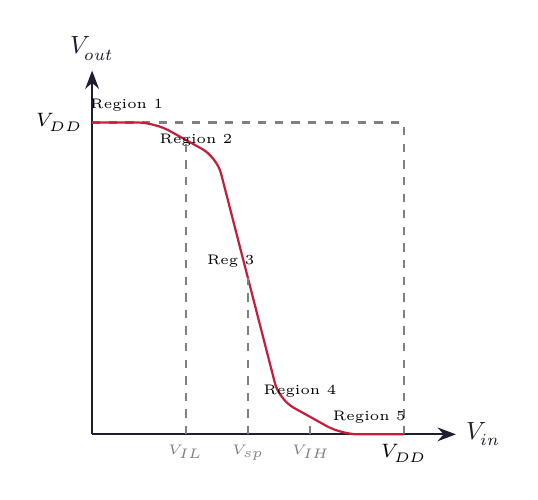
\begin{tikzpicture}[scale=1.1, thick, font=\small]
  % Axes
  \draw[arrow] (0, 0) -- (4.2, 0) node[right] {$V_{in}$};
  \draw[arrow] (0, 0) -- (0, 4.2) node[above] {$V_{out}$};
  
  % Limits
  \draw[dashed, gray] (3.6, 0) -- (3.6, 3.6);
  \draw[dashed, gray] (0, 3.6) -- (3.6, 3.6);
  \node[left, font=\scriptsize] at (0, 3.6) {$V_{DD}$};
  \node[below, font=\scriptsize] at (3.6, 0) {$V_{DD}$};

  % VTC Curve
  \draw[line, color=myred, rounded corners=6pt] (0, 3.6) -- (0.72, 3.6) -- (1.44, 3.2) -- (1.8, 1.8) -- (2.16, 0.4) -- (2.88, 0) -- (3.6, 0);

  % Regions labels
  \node[font=\tiny] at (0.4, 3.8) {Region 1};
  \node[font=\tiny] at (1.2, 3.4) {Region 2};
  \node[font=\tiny] at (1.6, 2.0) {Reg 3};
  \node[font=\tiny] at (2.4, 0.5) {Region 4};
  \node[font=\tiny] at (3.2, 0.2) {Region 5};

  % Critical Points (Slope = -1)
  % V_IL
  \draw[dashed, gray] (1.08, 0) node[below, font=\tiny] {$V_{IL}$} -- (1.08, 3.45);
  % V_IH
  \draw[dashed, gray] (2.52, 0) node[below, font=\tiny] {$V_{IH}$} -- (2.52, 0.15);
  % V_th (Switching Threshold)
  \draw[dashed, gray] (1.8, 0) node[below, font=\tiny] {$V_{sp}$} -- (1.8, 1.8);
\end{tikzpicture}
\end{tcolorbox}

\begin{enumerate}[label=\arabic*., leftmargin=*]
  \item \textbf{Region 1 ($0 \le V_{in} < V_{thn}$):} Input is low. nMOS is cut-off ($I_{Dn} = 0$). pMOS is ON in the linear region. $V_{out} = V_{DD}$.
  \item \textbf{Region 2 ($V_{thn} \le V_{in} < V_{sp}$):} nMOS turns ON in saturation ($V_{DSn} > V_{GSn} - V_{thn}$). pMOS is ON in linear region. $V_{out}$ begins to drop.
  \item \textbf{Region 3 ($V_{in} = V_{sp}$):} Switching threshold. Both nMOS and pMOS are in saturation. The output drops steeply.
  \item \textbf{Region 4 ($V_{sp} < V_{in} \le V_{DD} - |V_{thp}|$):} nMOS is ON in linear region. pMOS is ON in saturation region.
  \item \textbf{Region 5 ($V_{in} > V_{DD} - |V_{thp}|$):} Input is high. pMOS is cut-off ($I_{Dp} = 0$). nMOS is ON in linear region. $V_{out} = 0\,\text{V}$.
\end{enumerate}

\subsection{Derivation of Switching Threshold ($V_{sp}$)}
The switching threshold (or gate threshold voltage $V_{sp}$) is defined as the point where $V_{in} = V_{out}$. In Region 3, both transistors are in saturation:
\begin{equation}
  I_{Dn} = I_{Dp} \implies \frac{1}{2} k_n \left( V_{sp} - V_{thn} \right)^2 = \frac{1}{2} k_p \left( V_{DD} - V_{sp} - |V_{thp}| \right)^2
\end{equation}
Taking the square root on both sides:
\begin{equation}
  \sqrt{k_n} \left( V_{sp} - V_{thn} \right) = \sqrt{k_p} \left( V_{DD} - V_{sp} - |V_{thp}| \right)
\end{equation}
Divide by $\sqrt{k_n}$ and define the ratio $r = \sqrt{k_p / k_n}$:
\begin{equation}
  V_{sp} - V_{thn} = r \left( V_{DD} - V_{sp} - |V_{thp}| \right)
\end{equation}
\begin{equation}
  V_{sp} (1 + r) = V_{thn} + r \left( V_{DD} - |V_{thp}| \right)
\end{equation}
\begin{equation}
  V_{sp} = \frac{V_{thn} + r \left( V_{DD} - |V_{thp}| \right)}{1 + r}
\end{equation}
For a \textbf{symmetric inverter} where $k_n = k_p \implies r = 1$, and $V_{thn} = |V_{thp}|$:
\begin{equation}
  V_{sp} = \frac{V_{DD}}{2}
\end{equation}
To achieve a symmetric inverter ($k_n = k_p$), since electron mobility $\mu_n \approx 2.5\mu_p$, we must scale the channel widths:
\begin{equation}
  \mu_n C_{ox} \frac{W_n}{L_n} = \mu_p C_{ox} \frac{W_p}{L_p} \implies \left(\frac{W}{L}\right)_p \approx 2.5 \left(\frac{W}{L}\right)_n
\end{equation}

\subsection{Noise Margins ($NM_H, NM_L$)}
Noise margin measures the allowable electrical noise voltage on input terminals before the gate output state becomes corrupted.

\textbf{Critical Voltages}:
\begin{itemize}[leftmargin=*, itemsep=3.5pt]
  \item $V_{IL}$ (Input Low Voltage): The highest input voltage interpreted as Logic '0' (where $dV_{out}/dV_{in} = -1$).
  \item $V_{IH}$ (Input High Voltage): The lowest input voltage interpreted as Logic '1' (where $dV_{out}/dV_{in} = -1$).
  \item $V_{OL}$ (Output Low Voltage): Static low output: $V_{OL} = 0\,\text{V}$ for CMOS.
  \item $V_{OH}$ (Output High Voltage): Static high output: $V_{OH} = V_{DD}$ for CMOS.
\end{itemize}

\textbf{Formulas}:
\begin{equation}
  NM_L = V_{IL} - V_{OL} = V_{IL}
\end{equation}
\begin{equation}
  NM_H = V_{OH} - V_{IH} = V_{DD} - V_{IH}
\end{equation}

\section{Alternative load Inverters}

Before static CMOS was standardized, alternative single-channel (nMOS-only) designs were used to avoid fabricating pMOS devices.

\begin{itemize}[leftmargin=*, itemsep=3.5pt]
  \item \textbf{Resistive-Load Inverter:} Uses a passive resistor $R_L$ as the pull-up load. Drawbacks: consumes a massive silicon area for high resistance; has static power dissipation when output is low ($I_{static} = V_{DD}/R_L$).
  \item \textbf{Enhancement-Load Inverter:} Uses an enhancement-mode nMOS transistor as a load (gate connected to $V_{DD}$ or drain). Drawbacks: Output high voltage is degraded ($V_{OH} = V_{DD} - V_{thn}$), and suffers from static power dissipation when $V_{out}$ is low.
  \item \textbf{Depletion-Load Inverter:} Uses a depletion-mode nMOS transistor (with gate shorted to source, $V_{GS}=0$) as a load. Acts as a constant current source, yielding a sharper VTC transition and full logic swing ($V_{OH} = V_{DD}$), but still has high static power dissipation when output is low.
\end{itemize}

\begin{tcolorbox}[tikzbox, title={CMOS vs Depletion-Load Inverter Comparison}]
\renewcommand{\arraystretch}{1.4}
\par\noindent
\begin{tabularx}{\linewidth}{|B{3.2cm}|Y|Y|}
\hline
\textbf{Feature} & \textbf{\color{myred}Static CMOS Inverter} & \textbf{\color{myteal}Depletion-Load Inverter} \\
\hline
\textbf{Device Count} & 2 (1 nMOS, 1 pMOS). & 2 (1 enhancement, 1 depletion nMOS). \\
\hline
\textbf{Logic Swing} & Full rail-to-rail swing ($0$ to $V_{DD}$). & High swing (nearly $0$ to $V_{DD}$). \\
\hline
\textbf{Static Power} & Zero (ignoring tiny leakage). & High (when $V_{out}$ is low). \\
\hline
\textbf{Transition Width} & Narrow, sharp drop. & Moderate. \\
\hline
\textbf{Fabrication} & High complexity (well formation). & Low complexity (single-channel). \\
\hline
\end{tabularx}
\tcbset{colbacktitle=mypurple, coltitle=white}
\end{tcolorbox}

\newpage
% ===============================================================================
% MANDATORY QUICK REVISION PAGE
% ===============================================================================
\begin{center}
  {\large\bfseries\color{myred} Quick Revision --- Module 4}\\[3pt]
  {\small\color{mydark} MOS \& CMOS Inverters (Static Characteristics) $|$ PE-EC603C}
\end{center}
\noindent{\color{myred}\rule{\linewidth}{1.2pt}}
\vspace{4pt}

\begin{tcolorbox}[formulabox, title={\textbf{Key Inverter Equations}}]
$$V_{sp} = \frac{V_{thn} + r(V_{DD} - |V_{thp}|)}{1 + r} \qquad \text{where} \ r = \sqrt{\frac{k_p}{k_n}} = \sqrt{\frac{\mu_p W_p L_n}{\mu_n W_n L_p}}$$
$$\text{Symmetric Inverter Width Ratio:} \quad \left(\frac{W}{L}\right)_p \approx 2.5 \left(\frac{W}{L}\right)_n \qquad V_{sp} = \frac{V_{DD}}{2}$$
$$NM_L = V_{IL} - V_{OL} = V_{IL} \qquad NM_H = V_{OH} - V_{IH} = V_{DD} - V_{IH}$$
\end{tcolorbox}

\begin{tcolorbox}[defbox, title={\textbf{One-Line Definitions}}]
\begin{itemize}[leftmargin=*, itemsep=2.5pt, topsep=0pt]
  \item \textbf{VTC:} Plot of output voltage against input voltage characterizing static gain and noise immunities.
  \item \textbf{Switching Threshold ($V_{sp}$):} Input voltage at which the output voltage equals the input voltage ($V_{in} = V_{out}$).
  \item \textbf{Noise Margin:} The maximum noise voltage that can be added to the input signal without corrupting the output logic state.
  \item \textbf{Symmetric Inverter:} An inverter with identical pull-up and pull-down strengths, placing $V_{sp}$ exactly at $V_{DD}/2$.
  \item \textbf{Static Power Dissipation:} Power consumed by the gate when inputs are static (non-switching).
  \item \textbf{Depletion Load:} An nMOS transistor with $V_{th} < 0$, configured with gate shorted to source to act as a current source.
\end{itemize}
\end{tcolorbox}

\begin{tcolorbox}[exambox, title={\textbf{Frequently Asked / Viva Questions}}]
\begin{enumerate}[topsep=0pt, label=\textbf{Q\arabic*.}, itemsep=5pt]
  \item \Q{Why is the static power dissipation of a CMOS inverter practically zero?}
    Because in either steady state (Input = '0' or Input = '1'), one of the two series transistors (either pMOS or nMOS) is completely cut off, presenting an open circuit. Consequently, no direct path exists from $V_{DD}$ to GND, and current flow is limited to subthreshold and junction leakages (picoamps).
  \item \Q{Derive the switching threshold $V_{sp}$ of a CMOS inverter.}
    Equating saturation currents $I_{Dn} = I_{Dp} \implies \frac{1}{2} k_n (V_{sp} - V_{thn})^2 = \frac{1}{2} k_p (V_{DD} - V_{sp} - |V_{thp}|)^2$. Taking the square root, collecting terms, and solving for $V_{sp}$ yields $V_{sp} = \frac{V_{thn} + r(V_{DD} - |V_{thp}|)}{1+r}$ where $r = \sqrt{k_p/k_n}$.
  \item \Q{How do we design a symmetric CMOS inverter and why is it preferred?}
    A symmetric inverter has $V_{sp} = V_{DD}/2$, which maximizes both noise margins ($NM_L = NM_H$) and balances rise and fall propagation delays. It is achieved by setting $k_n = k_p \implies \mu_n(W/L)_n = \mu_p(W/L)_p \implies (W/L)_p \approx 2.5(W/L)_n$.
  \item \Q{Define Noise Margin and write its formulas for a CMOS inverter.}
    Noise margin represents the gate's noise immunity. For CMOS, since $V_{OL}=0$ and $V_{OH}=V_{DD}$, the margins are $NM_L = V_{IL} - V_{OL} = V_{IL}$ and $NM_H = V_{OH} - V_{IH} = V_{DD} - V_{IH}$, where $V_{IL}$ and $V_{IH}$ are input voltages where the VTC slope $dV_{out}/dV_{in} = -1$.
  \item \Q{Explain the VTC region 3 of a CMOS inverter.}
    In Region 3, the input is close to $V_{DD}/2$. Both nMOS and pMOS are in saturation simultaneously, acting as high-impedance current sources. This creates a very high voltage gain ($dV_{out}/dV_{in} \ll -1$), causing a steep drop in $V_{out}$.
  \item \Q{What are the disadvantages of a resistive-load inverter?}
    First, it consumes static power ($P = V_{DD}^2/R_L$) whenever the output is low because the pull-down nMOS is ON. Second, to get low $V_{OL}$, $R_L$ must be very large (tens of $\text{k}\Omega$), which requires a massive surface area on silicon compared to a transistor.
  \item \Q{Why does an enhancement-load inverter suffer from degraded $V_{OH}$?}
    In an enhancement-load nMOS inverter, the load transistor turns OFF when the output rises to $V_{DD} - V_{thn}$ because its gate-source voltage drops below the threshold voltage. Thus, it cannot pull the output all the way up to $V_{DD}$.
  \item \Q{Explain the depletion-load inverter and its advantage over resistive-load.}
    The depletion-load inverter uses a depletion-mode nMOS with $V_{th} < 0$ and gate shorted to source ($V_{GS}=0$). It behaves as a constant current source rather than a passive resistor, which pulls the output up to the full $V_{DD}$ and yields a sharper VTC transition.
  \item \Q{If a CMOS inverter has $V_{DD} = 3.3\,\text{V}$, $V_{thn} = 0.7\,\text{V}$, $|V_{thp}| = 0.8\,\text{V}$, and $r = 1.0$, calculate $V_{sp}$.}\\
    Using the formula: $V_{sp} = \frac{V_{thn} + r(V_{DD} - |V_{thp}|)}{1+r} = \frac{0.7 + 1.0 \times (3.3 - 0.8)}{1 + 1} = \frac{0.7 + 2.5}{2} = 1.6\,\text{V}$.
  \item \Q{How does noise margin scale when we reduce the supply voltage $V_{DD}$?}
    As $V_{DD}$ scales down, the total transition range of the VTC shrinks. Since critical points $V_{IL}$ and $V_{IH}$ scale proportionally with $V_{DD}$, the absolute noise margins ($NM_L, NM_H$) decrease, making the circuit more sensitive to external electrical noise.
\end{enumerate}
\end{tcolorbox}


% -- Module 5 -----------------------------------------------------------------
\modulestart{5}{CMOS Combinational Logic Gates}

\section{CMOS Combinational Logic Gates}
% ===============================================================================

Combinational logic circuits in CMOS are built using complementary networks: a Pull-Up Network (PUN) composed of pMOS transistors and a Pull-Down Network (PDN) composed of nMOS transistors.

\subsection{Static NAND \& NOR Gates}
Static CMOS gates are complementary. For any boolean function, if the nMOS PDN implements the function in its uncomplemented form, the pMOS PUN implements the dual function.

\begin{itemize}[leftmargin=*, itemsep=4pt]
  \item \textbf{2-Input NAND Gate:}
    \begin{itemize}
      \item \textbf{PDN:} Two nMOS transistors connected in series. Both must be ON ($A = B = 1$) to pull the output to GND.
      \item \textbf{PUN:} Two pMOS transistors connected in parallel. If either input is low ($A=0$ or $B=0$), at least one pMOS pulls the output to $V_{DD}$.
      \item \textbf{Sizing:} Since two series nMOS transistors double the pull-down path resistance, each nMOS must be sized $2W_n$ to achieve the same drive current as a standard inverter. The parallel pMOS transistors remain $W_p \approx 2.5W_n$.
    \end{itemize}
  \item \textbf{2-Input NOR Gate:}
    \begin{itemize}
      \item \textbf{PDN:} Two nMOS transistors connected in parallel. If either input is high, the output is pulled to GND.
      \item \textbf{PUN:} Two pMOS transistors connected in series. Both inputs must be low to pull the output to $V_{DD}$.
      \item \textbf{Sizing:} Since two series pMOS transistors double the pull-up path resistance, each pMOS must be sized $2W_p \approx 5W_n$ to match a standard inverter. The parallel nMOS transistors remain $W_n$.
    \end{itemize}
\end{itemize}

\subsection{Complex Logic Gates (AOI \& OAI)}
Complex gates implement multiple logic operations in a single physical gate, reducing transistor count, parasitics, and propagation delay.
\begin{itemize}[leftmargin=*, itemsep=3.5pt]
  \item \textbf{AND-OR-INVERT (AOI):} Implements the function $Y = \overline{(A \cdot B) + C}$.
    \begin{itemize}
      \item \textbf{PDN (AND-OR):} Transistors $A$ and $B$ are in series, and this group is in parallel with transistor $C$.
      \item \textbf{PUN (OR-AND):} Dual network: Transistors $A$ and $B$ are in parallel, and this group is in series with transistor $C$.
    \end{itemize}
  \item \textbf{OR-AND-INVERT (OAI):} Implements the function $Y = \overline{(A + B) \cdot C}$.
    \begin{itemize}
      \item \textbf{PDN (OR-AND):} Transistors $A$ and $B$ are in parallel, and this group is in series with transistor $C$.
      \item \textbf{PUN (AND-OR):} Dual network: Transistors $A$ and $B$ are in series, and this group is in parallel with transistor $C$.
    \end{itemize}
\end{itemize}

% ===============================================================================
\section{Switching \& Transient Characteristics}
% ===============================================================================

The dynamic performance of a digital gate is determined by how quickly it can charge and discharge its output load capacitance.

\subsection{Propagation Delay Derivation ($t_{pHL}, t_{pLH}$)}
Using an equivalent RC model, the propagation delay represents the time taken for the output to reach 50\% of its final value after the input crosses its 50\% value.

Consider a capacitor $C_L$ discharging from $V_{DD}$ to 0 through an nMOS transistor. The transient discharge voltage is governed by the differential equation:
\begin{equation}
  i_D(t) = -C_L \frac{d V_{out}(t)}{d t}
\end{equation}

For a simplified analysis, we approximate the transistor as a constant equivalent resistance $R_{on,n}$ during the transition:
\begin{equation}
  V_{out}(t) = V_{DD} e^{-t / \tau_n} \qquad \text{where} \ \tau_n = R_{on,n} C_L
\end{equation}

To find the high-to-low propagation delay $t_{pHL}$, we solve for $V_{out}(t_{pHL}) = 0.5 V_{DD}$:
\begin{equation}
  0.5 V_{DD} = V_{DD} e^{-t_{pHL} / \tau_n} \implies e^{t_{pHL} / \tau_n} = 2
\end{equation}
\begin{equation}
  t_{pHL} = \ln(2) \tau_n = \ln(2) R_{on,n} C_L \approx 0.69 R_{on,n} C_L
\end{equation}

Similarly, the low-to-high propagation delay $t_{pLH}$ for charging $C_L$ through the pMOS pull-up network is:
\begin{equation}
  t_{pLH} = \ln(2) \tau_p = \ln(2) R_{on,p} C_L \approx 0.69 R_{on,p} C_L
\end{equation}

The average propagation delay $t_p$ of the gate is:
\begin{equation}
  t_p = \frac{t_{pHL} + t_{pLH}}{2}
\end{equation}

\subsection{Rise and Fall Times ($t_r, t_f$)}
\begin{itemize}[leftmargin=*, itemsep=3.5pt]
  \item \textbf{Fall Time ($t_f$):} Time required for the output to drop from 90\% to 10\% of its initial value ($V_{DD}$).
    \begin{equation}
      t_f = t_{10\%} - t_{90\%} = \tau_n \ln(0.1) - \tau_n \ln(0.9) = \tau_n \ln\left(\frac{0.9}{0.1}\right) = \tau_n \ln(9) \approx 2.2 R_{on,n} C_L
    \end{equation}
  \item \textbf{Rise Time ($t_r$):} Time required for the output to rise from 10\% to 90\% of its final value ($V_{DD}$).
    \begin{equation}
      t_r \approx 2.2 R_{on,p} C_L
    \end{equation}
\end{itemize}

\subsection{Parasitic Capacitance Components}
The total load capacitance $C_L$ consists of:
\begin{equation}
  C_L = C_{gate} + C_{diff} + C_{wire}
\end{equation}
\begin{enumerate}[label=\arabic*., leftmargin=*]
  \item \textbf{Gate Capacitance ($C_{gate}$):} The input capacitance of the succeeding logic gates.
  \item \textbf{Diffusion Capacitance ($C_{diff}$):} The drain junction capacitances of the driving gate itself, comprising area and sidewall components: $C_{diff} = A_D C_{j} + P_D C_{jsw}$.
  \item \textbf{Routing/Wire Capacitance ($C_{wire}$):} The capacitance of the metal interconnect lines linking the gates.
\end{enumerate}

% ===============================================================================
\section{Dynamic CMOS Logic Circuits}
% ===============================================================================

Dynamic logic circuits rely on the temporary storage of charge on a high-impedance node rather than continuous static connections.

\subsection{Dynamic Gate Principle and Operation}
A dynamic gate consists of a precharge pMOS ($M_{pre}$), an evaluate nMOS ($M_{eval}$), and an nMOS pull-down logic network (PDN). Its operation is split into two phases controlled by the clock ($\Phi$):

\begin{enumerate}[label=\arabic*., leftmargin=*]
  \item \textbf{Precharge Phase ($\Phi = 0$):}
    \begin{itemize}
      \item $M_{pre}$ is turned ON; $M_{eval}$ is turned OFF.
      \item The path to GND is blocked. The output node charge capacitance $C_L$ charges to $V_{DD}$.
      \item Output = High ('1') regardless of the inputs to the PDN.
    \end{itemize}
  \item \textbf{Evaluation Phase ($\Phi = 1$):}
    \begin{itemize}
      \item $M_{pre}$ is turned OFF; $M_{eval}$ is turned ON.
      \item If the input combination creates a conducting path through the PDN, the output node discharges to GND (Output = '0').
      \item If the PDN is non-conducting, the output node remains at its precharged value $V_{DD}$ via stored charge on $C_L$ (Output = '1').
    \end{itemize}
\end{enumerate}

\subsection{Problems in Dynamic Logic}
Despite having fewer transistors ($N+2$ instead of $2N$) and high speed, dynamic logic suffers from several severe physical issues:

\begin{itemize}[leftmargin=*, itemsep=4pt]
  \item \textbf{Charge Leakage:} During the evaluation phase, if the output node is left floating at $V_{DD}$, leakage currents (subthreshold leakage through the PDN and reverse-biased junction leakage) slowly discharge $C_L$, degrading the logic level. This limits the minimum clock operating frequency.
  \item \textbf{Charge Sharing:}
    If the output is precharged to $V_{DD}$ and an internal node capacitance $C_{int}$ is initially discharged, turning on a subset of the PDN that does not lead to GND will cause the charge on $C_L$ to redistribute with $C_{int}$.
    The final output voltage drops to:
    \begin{equation}
      V_{out} = V_{DD} \left( \frac{C_L}{C_L + C_{int}} \right)
    \end{equation}
    If $V_{out}$ drops below the switching threshold of the next gate, a logic error occurs.
  \item \textbf{Cascading Problem:}
    When dynamic gates are directly cascaded, during precharge, both stage outputs are $V_{DD}$. When evaluation begins ($\Phi = 1$), the inputs to Stage 2 are initially '1'.
    Before Stage 1 can evaluate and drop its output to '0', Stage 2 sees a '1' at its input and begins to discharge its precharged node. Once Stage 2 discharges, it cannot recover since the precharge transistor is OFF. This is a severe race condition.
\end{itemize}

\subsection{Domino Logic}
Domino CMOS logic solves the cascading problem by inserting a static CMOS inverter at the output of every dynamic stage.

\begin{tcolorbox}[defbox, title={\textbf{Domino Logic Mechanism}}]
During precharge ($\Phi = 0$), the dynamic node is charged to $V_{DD}$, making the static inverter output 0. Since the inverter output is 0, the nMOS inputs of all subsequent stages are held OFF. When evaluation begins ($\Phi=1$), the nodes evaluate sequentially like falling dominoes, preventing premature discharge.
\end{tcolorbox}

To prevent charge leakage and charge sharing, a weak pMOS feedback transistor (called a \textbf{keeper}) is added, controlled by the inverter output, to hold the dynamic node at $V_{DD}$ when it is floating.

\begin{tcolorbox}[tikzbox, title={Domino CMOS Logic Gate Circuit Diagram}]
\centering
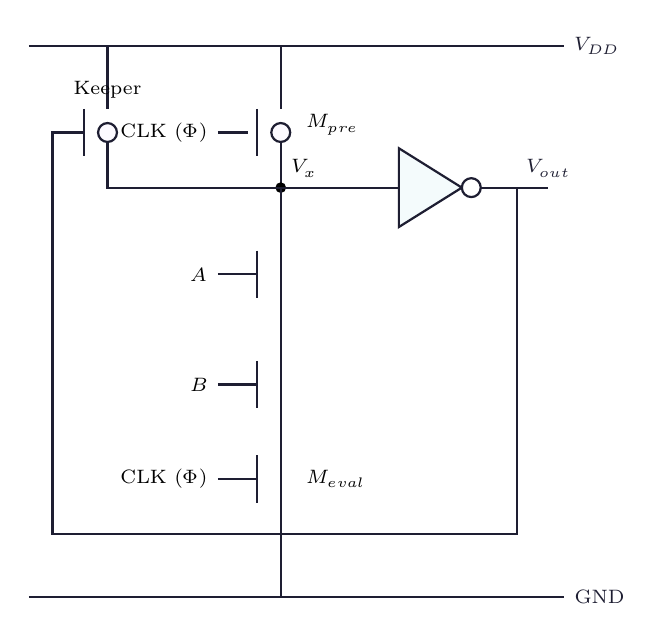
\begin{tikzpicture}[scale=1.0, thick, font=\small]
  % VDD and GND rails
  \draw[line] (-3.2, 4) -- (3.6, 4) node[right, font=\scriptsize] {$V_{DD}$};
  \draw[line] (-3.2, -3) -- (3.6, -3) node[right, font=\scriptsize] {GND};

  % Precharge pMOS (M_pre) at x=0
  \draw[line] (0, 4) -- (0, 3.2);
  \draw[draw=mydark, fill=hdrpurple!20] (0, 2.9) circle (0.12);
  \draw[line] (-0.3, 3.2) -- (-0.3, 2.6); % Gate plate
  \draw[line] (-0.8, 2.9) -- (-0.42, 2.9); % Gate input
  \node[left, font=\scriptsize] at (-0.8, 2.9) {CLK ($\Phi$)};
  \draw[line] (0, 2.78) -- (0, 2.2);
  \node[right, font=\scriptsize] at (0.2, 3.0) {$M_{pre}$};

  % Dynamic Node V_x
  \filldraw (0, 2.2) circle (1.5pt) node[above right, font=\scriptsize] {$V_x$};
  
  % Pull Down Logic Network (PDN) at x=0
  \draw[line] (0, 2.2) -- (0, 1.4);
  % nMOS 1 (Input A)
  \draw[line] (-0.3, 1.4) -- (-0.3, 0.8);
  \draw[line] (-0.8, 1.1) -- (-0.3, 1.1);
  \node[left, font=\scriptsize] at (-0.8, 1.1) {$A$};
  \draw[line] (0, 1.4) -- (0, 0.8);
  
  % nMOS 2 (Input B)
  \draw[line] (0, 0.8) -- (0, 0);
  \draw[line] (-0.3, 0) -- (-0.3, -0.6);
  \draw[line] (-0.8, -0.3) -- (-0.3, -0.3);
  \node[left, font=\scriptsize] at (-0.8, -0.3) {$B$};
  \draw[line] (0, 0) -- (0, -0.6);
  
  % Evaluate nMOS (M_eval) at x=0
  \draw[line] (0, -0.6) -- (0, -1.2);
  \draw[line] (-0.3, -1.2) -- (-0.3, -1.8);
  \draw[line] (-0.8, -1.5) -- (-0.3, -1.5);
  \node[left, font=\scriptsize] at (-0.8, -1.5) {CLK ($\Phi$)};
  \draw[line] (0, -1.2) -- (0, -1.8);
  \draw[line] (0, -1.8) -- (0, -3);
  \node[right, font=\scriptsize] at (0.2, -1.5) {$M_{eval}$};

  % Weak Keeper pMOS (Feedback) at x=-2.2
  \draw[line] (-2.2, 4) -- (-2.2, 3.2);
  \draw[draw=mydark, fill=hdrpurple!20] (-2.2, 2.9) circle (0.12);
  \draw[line] (-2.5, 3.2) -- (-2.5, 2.6); % Gate plate
  \draw[line] (-2.2, 2.78) -- (-2.2, 2.2) -- (0, 2.2); % Drain to Vx
  \node[above, font=\scriptsize] at (-2.2, 3.2) {Keeper};

  % Connection to Static Inverter
  \draw[line] (0, 2.2) -- (1.5, 2.2);
  
  % Inverter Block
  \draw[draw=mydark, fill=hdrteal!30] (1.5, 1.7) -- (2.3, 2.2) -- (1.5, 2.7) -- cycle;
  \draw[draw=mydark, fill=white] (2.42, 2.2) circle (0.12);
  \draw[line] (2.54, 2.2) -- (3.4, 2.2) node[above, font=\scriptsize] {$V_{out}$};

  % Feedback connection from V_out to Keeper gate
  \draw[line] (3.0, 2.2) -- (3.0, -2.2) -- (-2.9, -2.2) -- (-2.9, 2.9) -- (-2.5, 2.9);
\end{tikzpicture}
\end{tcolorbox}

\subsection{NORA Logic}
NORA (No-Race) CMOS logic avoids the static inverter delay of Domino logic by alternating dynamic blocks of opposite logic structures:
\begin{itemize}[leftmargin=*, itemsep=3.5pt]
  \item \textbf{n-tree block:} Uses an nMOS PDN. Precharges to $V_{DD}$ ($\Phi = 0$) and evaluates to GND ($\Phi = 1$).
  \item \textbf{p-tree block:} Uses a pMOS PUN. Precharges to GND ($\Phi = 0$ using an nMOS precharge) and evaluates to $V_{DD}$ ($\Phi = 1$ using a pMOS evaluation transistor).
  \item By cascading an n-tree stage directly into a p-tree stage, the cascading race is eliminated because the outputs are in opposite precharged states.
\end{itemize}

% ===============================================================================
\section{CMOS Sequential Logic Circuits}
% ===============================================================================

Sequential logic circuits use feedback loop topologies to store state.

\subsection{SR Latch}
The SR latch is a bistable circuit. The NAND-based implementation uses cross-coupled NAND gates.
\begin{itemize}[leftmargin=*, itemsep=3pt]
  \item When $S' = 0, R' = 1$, the latch sets ($Q=1, Q'=0$).
  \item When $S' = 1, R' = 0$, the latch resets ($Q=0, Q'=1$).
  \item When $S' = 1, R' = 1$, the latch holds its previous state.
  \item When $S' = 0, R' = 0$, both outputs go to 1 (invalid state).
\end{itemize}

\subsection{D Latch (Transmission Gate Based)}
A D Latch is level-sensitive. It is built using Transmission Gates (TGs) and cross-coupled inverters.
\begin{itemize}[leftmargin=*, itemsep=3.5pt]
  \item A TG consists of an nMOS and a pMOS connected in parallel, controlled by complementary clocks ($CLK$ and $CLK'$). It acts as an ideal bilateral switch with zero voltage degradation.
  \item \textbf{Transparent Mode ($CLK = 1$):} The input TG is ON, passing input $D$ to the output ($Q = D$). The feedback loop is open because the feedback TG is OFF.
  \item \textbf{Hold Mode ($CLK = 0$):} The input TG is OFF, isolating the storage node. The feedback TG is ON, closing the cross-coupled inverter loop to hold the stored state indefinitely.
\end{itemize}

\subsection{D Flip-flop (Master-Slave Configuration)}
An edge-triggered D flip-flop is constructed by cascading two D latches in a Master-Slave structure controlled by complementary clock phases:
\begin{itemize}[leftmargin=*, itemsep=3.5pt]
  \item \textbf{Master Latch:} Level-sensitive, transparent when $CLK=0$, holds when $CLK=1$.
  \item \textbf{Slave Latch:} Level-sensitive, holds when $CLK=0$, transparent when $CLK=1$.
  \item \textbf{Overall Operation:}
    \begin{itemize}
      \item When $CLK = 0$, the Master is transparent (samples input $D$), and the Slave is in hold mode (retains previous state).
      \item On the rising edge of $CLK$ ($0 \to 1$), the Master goes into hold mode, locking the sampled input value. Concurrently, the Slave becomes transparent, passing the locked Master output to the final output $Q$.
      \item This creates a negative-edge or positive-edge triggered behavior depending on clock routing.
    \end{itemize}
\end{itemize}

\newpage
% ===============================================================================
% MANDATORY QUICK REVISION PAGE
% ===============================================================================
\begin{center}
  {\large\bfseries\color{myred} Quick Revision --- Module 5}\\[3pt]
  {\small\color{mydark} Dynamic CMOS Circuits \& Sequential Logic $|$ PE-EC603C}
\end{center}
\noindent{\color{myred}\rule{\linewidth}{1.2pt}}
\vspace{4pt}

\begin{tcolorbox}[formulabox, title={\textbf{Key Equations}}]
$$\text{Propagation Delay:} \quad t_{pHL} \approx 0.69 R_{on,n} C_L \qquad t_{pLH} \approx 0.69 R_{on,p} C_L$$
$$\text{Rise \& Fall Times:} \quad t_f \approx 2.2 R_{on,n} C_L \qquad t_r \approx 2.2 R_{on,p} C_L$$
$$\text{Charge Sharing final voltage:} \quad V_{out,final} = V_{DD} \left( \frac{C_L}{C_L + C_{int}} \right)$$
$$\text{2-Input NAND Sizing:} \quad W_n' = 2W_n, \ W_p' = W_p \qquad \text{2-Input NOR Sizing:} \quad W_n' = W_n, \ W_p' = 2W_p$$
\end{tcolorbox}

\begin{tcolorbox}[defbox, title={\textbf{One-Line Definitions}}]
\begin{itemize}[leftmargin=*, itemsep=2.5pt, topsep=0pt]
  \item \textbf{AOI Gate:} A static CMOS gate implementing series-parallel logic that ANDs, ORs, then inverts the inputs.
  \item \textbf{Propagation Delay:} Average time required for output signal transitions to reach 50\% of their value relative to the input.
  \item \textbf{Dynamic CMOS Logic:} A class of logic gates using clock phases to precharge and evaluate logic on temporary capacitances.
  \item \textbf{Charge Sharing:} Charge redistribution between a floating node and internal node capacitances, causing voltage drops.
  \item \textbf{Domino Logic:} Dynamic CMOS logic configuration with a static inverter at the output to ensure stable cascaded evaluation.
  \item \textbf{Keeper Transistor:} A weak feedback transistor used to combat leakage and noise on dynamic high-impedance nodes.
  \item \textbf{Transmission Gate:} A bilateral analog switch consisting of parallel nMOS and pMOS transistors driven by complementary clocks.
\end{itemize}
\end{tcolorbox}

\begin{tcolorbox}[exambox, title={\textbf{Frequently Asked / Viva Questions}}]
\begin{enumerate}[topsep=0pt, label=\textbf{Q\arabic*.}, itemsep=5pt]
  \item \Q{Why does a series transistor stack require width scaling in static CMOS?}
    In static CMOS, putting transistors in series increases the effective channel length, doubling the resistance for two transistors. To maintain the same drive current (speed) as a standard inverter, the width $W$ of each series transistor must be doubled.
  \item \Q{Derive the propagation delay expression $t_{pHL} = 0.69 R_{on,n} C_L$ using the RC model.}
    For an RC discharge circuit, $V_{out}(t) = V_{DD} e^{-t/RC}$. The propagation delay $t_{pHL}$ is the time when $V_{out}(t_{pHL}) = 0.5 V_{DD} \implies 0.5 V_{DD} = V_{DD} e^{-t_{pHL}/RC} \implies e^{-t_{pHL}/RC} = 1/2 \implies t_{pHL} = RC \ln(2) \approx 0.69 R_{on,n} C_L$.
  \item \Q{What are the primary differences between Rise/Fall time and Propagation Delay?}
    Rise/Fall time ($t_r/t_f$) is the time taken for a single signal to transition between 10\% and 90\% of its peak amplitude. Propagation delay ($t_{pLH}/t_{pHL}$) measures the time difference between the input crossing 50\% and the output crossing 50\% during a transition.
  \item \Q{Explain the precharge and evaluation phases in dynamic CMOS logic.}
    During precharge ($\text{CLK} = 0$), the precharge pMOS is ON, charging the output node to $V_{DD}$, while the evaluate nMOS is OFF. During evaluation ($\text{CLK} = 1$), the precharge pMOS is OFF, the evaluate nMOS is ON, and the output node either discharges to GND or stays high based on the PDN logic state.
  \item \Q{Why cannot raw dynamic CMOS gates be cascaded directly?}
    During precharge, outputs of all stages are high. When evaluation starts, the first stage's output takes a finite time to drop to 0. During this brief interval, the second stage sees a high input and discharges its node prematurely. This discharge is irreversible during that evaluation phase.
  \item \Q{How does Domino CMOS logic solve the cascading problem?}
    Domino logic places a static inverter after the dynamic node. During precharge, the dynamic node is high, making the inverter output 0. Thus, the succeeding stage nMOS inputs are held at 0, preventing them from discharging until the first stage has evaluated and its output transitions.
  \item \Q{What is the function of a keeper transistor in Domino logic?}
    The keeper is a weak pMOS transistor whose gate is driven by the output inverter. When the dynamic node is precharged and remains high, the inverter output is low, turning the keeper ON to pull the node to $V_{DD}$. This counters subthreshold leakage and charge sharing.
  \item \Q{Explain charge sharing in dynamic CMOS and how to mitigate it.}
    Charge sharing occurs when a precharged output node redistributes its charge with internal node capacitances in the PDN when some input switches. It causes the output voltage to drop. Mitigation techniques include adding a keeper transistor or precharging internal nodes to $V_{DD}$ during the precharge phase.
  \item \Q{What is NORA logic and how does it differ from Domino logic?}
    NORA (No-Race) logic alternates n-tree and p-tree dynamic stages rather than using static inverters between stages. The n-tree stages precharge to $V_{DD}$ and evaluate to GND, while the p-tree stages precharge to GND and evaluate to $V_{DD}$, allowing direct cascading.
  \item \Q{Describe the structure and advantage of a Transmission Gate (TG).}
    A TG consists of an nMOS and pMOS in parallel with complementary clock controls. Its main advantage is that it passes a full logic swing (both strong '0' and strong '1') without the threshold voltage drop ($V_{th}$) associated with single-transistor pass logic.
\end{enumerate}
\end{tcolorbox}

\begin{tcolorbox}[tikzbox, title={Static CMOS vs. Dynamic CMOS Logic}]
\renewcommand{\arraystretch}{1.4}
\par\noindent
\begin{tabularx}{\linewidth}{|B{3.2cm}|Y|Y|}
\hline
\textbf{Feature} & \textbf{\color{myred}Static CMOS} & \textbf{\color{myteal}Dynamic CMOS} \\
\hline
\textbf{Transistor Count} & $2N$ transistors (high area). & $N + 2$ transistors (low area). \\
\hline
\textbf{Static Power} & Virtually zero. & Virtually zero. \\
\hline
\textbf{Input Capacitance} & High (gates of both nMOS \& pMOS). & Low (gate of nMOS only). \\
\hline
\textbf{Speed} & Moderate. & High (lower parasitic capacitances). \\
\hline
\textbf{Sensitivity to Noise} & Low (high noise margins). & High (sensitive to leakage \& sharing). \\
\hline
\textbf{Clocking} & No clock required. & Requires a continuous clock signal. \\
\hline
\end{tabularx}
\end{tcolorbox}


% -- Module 6 -----------------------------------------------------------------
\modulestart{6}{Transistor Sizing \& Buffer Chains}

\section{Transistor Sizing \& Buffer Chains}
% ===============================================================================

To optimize circuit delay, transistors must be sized appropriately based on their load.

\subsection{Transistor Sizing Principles}
For a CMOS inverter, matching the pull-up and pull-down strengths requires:
\begin{equation}
  \beta_p = \beta_n \implies \mu_p C_{ox} \frac{W_p}{L_p} = \mu_n C_{ox} \frac{W_n}{L_n} \implies W_p \approx r \cdot W_n
\end{equation}
where $r = \mu_n / \mu_p$ is typically $2.5$ for silicon. In complex logic paths with $N$ series transistors, the channel width of each device must be increased to $N \cdot W$ to keep the path resistance equivalent to a single transistor of width $W$.

\subsection{Driving Large Capacitive Loads (Inverter Chain)}
When a small gate (input capacitance $C_{in}$) must drive a massive capacitive load $C_L$ (e.g., an output pad or global clock bus), using a single gate results in a very large delay. Instead, we cascade a chain of $N$ inverters, where each stage is scaled up by a constant factor $f$ relative to the preceding stage.

\begin{tcolorbox}[defbox, title={\textbf{Inverter Chain Sizing Model}}]
Let $C_{in, k}$ be the input capacitance of the $k$-th inverter. The scaling factor is:
\begin{equation}
  f = \frac{C_{in, k+1}}{C_{in, k}} \qquad \text{for} \ k = 1, \dots, N
\end{equation}
The total path sizing ratio is:
\begin{equation}
  F = \frac{C_L}{C_{in, 1}} = f^N
\end{equation}
\end{tcolorbox}

The total propagation delay of the chain is the sum of the delays of the $N$ stages. Assuming the delay of a standard inverter driving an identical load is $\tau_0$, the total delay is:
\begin{equation}
  t_{path} = N \cdot f \cdot \tau_0 = N \cdot \left(\frac{C_L}{C_{in, 1}}\right)^{1/N} \tau_0
\end{equation}

To find the optimal value of $N$ that minimizes the delay, we differentiate $t_{path}$ with respect to $N$ and set it to zero:
\begin{equation}
  \frac{d t_{path}}{d N} = 0 \implies f = e \approx 2.718
\end{equation}
In practical layout design, a sizing factor of $f \approx 3$ to $4$ is used to save area and power with minimal delay penalty. The optimal number of stages is:
\begin{equation}
  N = \ln(F) = \ln\left( \frac{C_L}{C_{in, 1}} \right)
\end{equation}

% ===============================================================================
\section{CMOS Power Dissipation}
% ===============================================================================

Power dissipation in CMOS circuits is divided into three components:
\begin{equation}
  P_{total} = P_{dynamic} + P_{short-circuit} + P_{static}
\end{equation}

\subsection{Dynamic Power Dissipation (\texorpdfstring{$P_{dynamic}$}{P\_dynamic})}
Dynamic power is consumed when the circuit switches states, charging and discharging node capacitances.

\begin{tcolorbox}[formulabox, title={\textbf{Dynamic Power Derivation}}]
During a low-to-high transition, the energy drawn from the power supply $V_{DD}$ is:
\begin{equation}
  E_{supply} = \int_{0}^{\infty} i_{supply}(t) V_{DD} \, d t = V_{DD} \int_{0}^{\infty} C_L \frac{d V_{out}}{d t} \, d t = C_L V_{DD}^2
\end{equation}
The energy stored in the capacitor at the end of the transition is:
\begin{equation}
  E_{cap} = \frac{1}{2} C_L V_{DD}^2
\end{equation}
The remaining half of the energy ($E_{diss, p} = \frac{1}{2} C_L V_{DD}^2$) is dissipated as heat in the pMOS pull-up path. During the high-to-low transition, no energy is drawn from the supply, and the stored capacitor energy is dissipated in the nMOS pull-down path ($E_{diss, n} = \frac{1}{2} C_L V_{DD}^2$).

Thus, the total energy dissipated per switching cycle (one $0 \to 1$ and one $1 \to 0$ transition) is:
\begin{equation}
  E_{cycle} = E_{diss, p} + E_{diss, n} = C_L V_{DD}^2
\end{equation}
If the circuit switches at a clock frequency $f$ with an activity factor $\alpha$ (probability of a transition occurring per cycle), the average dynamic power is:
\begin{equation}
  P_{dynamic} = \alpha C_L V_{DD}^2 f
\end{equation}
\end{tcolorbox}

\subsection{Short-Circuit Power Dissipation (\texorpdfstring{$P_{short-circuit}$}{P\_short-circuit})}
During input transitions, when the input voltage $V_{in}$ is between $V_{thn}$ and $V_{DD} - |V_{thp}|$, both the nMOS and pMOS transistors are simultaneously ON. This creates a direct conductive path from $V_{DD}$ to GND, resulting in a short-circuit current spike $I_{sc}$.

\textbf{Minimization:} Short-circuit power is minimized by keeping input signal rise and fall times very sharp, ensuring the transistors remain in the active overlap region for a negligible fraction of time.

\subsection{Static Power Dissipation (\texorpdfstring{$P_{static}$}{P\_static})}
Static power is consumed when the inputs are constant (no switching activity):
\begin{equation}
  P_{static} = I_{leak} \cdot V_{DD}
\end{equation}
The leakage current $I_{leak}$ consists of:
\begin{enumerate}[label=\arabic*., leftmargin=*]
  \item \textbf{Subthreshold Leakage:} Current flowing from drain to source when $V_{GS} < V_{th}$, which increases exponentially as technology scales down and $V_{th}$ is lowered.
  \item \textbf{Gate Oxide Leakage:} Tunneling current through the extremely thin gate oxide dielectric.
  \item \textbf{Junction Leakage:} Reverse-biased PN junction leakage between diffusion wells and substrate.
\end{enumerate}

\subsection{Latch-Up and Prevention}
Latch-up is a critical failure mode in CMOS circuits where a low-impedance path is established between $V_{DD}$ and GND, leading to massive current draw and permanent device destruction.

\begin{itemize}[leftmargin=*, itemsep=4pt]
  \item \textbf{Cause:} It is caused by the accidental triggering of parasitic bipolar transistors (a PNP transistor formed by p+ source/drain, n-well, and p-substrate; and an NPN transistor formed by n+ source/drain, p-substrate, and n-well) that form a back-to-back SCR (Silicon Controlled Rectifier) feedback loop.
  \item \textbf{Mitigation Techniques:}
    \begin{itemize}[leftmargin=*, itemsep=2.5pt, topsep=2pt]
      \item \textbf{Guard Rings:} Place heavily doped $n^+$ rings in the n-well connected to $V_{DD}$, and $p^+$ rings in the p-substrate connected to GND to collect stray carriers before they reach the bases of the parasitic BJTs.
      \item \textbf{Substrate Contacts:} Maximize substrate/well taps close to the source contacts of transistors to keep the local well resistance low ($R_{well}, R_{sub} \approx 0$), preventing base-emitter forward bias.
      \item \textbf{Trench Isolation:} Use Shallow Trench Isolation (STI) between nMOS and pMOS to physically block the parasitic BJT path.
    \end{itemize}
\end{itemize}

% ===============================================================================
\section{Layout and Design Rules}
% ===============================================================================

Physical layout translates the schematic into geometric masks for chip fabrication.

\subsection{Stick Diagrams}
A stick diagram is a simplified topological representation of a layout, showing the relative placement and interconnection of layers without absolute dimensions.

\begin{tcolorbox}[defbox, title={\textbf{Stick Diagram Color Codes}}]
\begin{itemize}[leftmargin=*, itemsep=2.5pt, topsep=0pt]
  \item \textbf{\color{myteal}Blue (Metal 1):} Power rails ($V_{DD}$, GND) and routing connections.
  \item \textbf{\color{myred}Red (Polysilicon):} Gate electrodes and input signal lines.
  \item \textbf{\color{mygreen}Green (n-Diffusion):} Active areas for nMOS transistors.
  \item \textbf{\color{myamber}Amber/Yellow (p-Diffusion):} Active areas for pMOS transistors.
  \item \textbf{Black Cross / Dot:} Contact cuts connecting different layers.
\end{itemize}
\end{tcolorbox}

\begin{tcolorbox}[tikzbox, title={Stick Diagram of a 2-Input CMOS NAND Gate}]
\centering
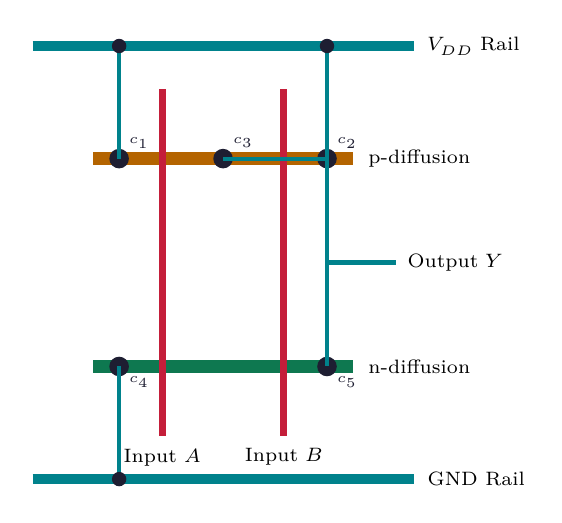
\begin{tikzpicture}[scale=1.1, thick, font=\small]
  % Rails (Metal 1 - Blue/Teal)
  \draw[draw=myteal, line width=3.5pt] (-2.2, 2.5) -- (2.2, 2.5) node[right, font=\scriptsize] {$V_{DD}$ Rail};
  \draw[draw=myteal, line width=3.5pt] (-2.2, -2.5) -- (2.2, -2.5) node[right, font=\scriptsize] {GND Rail};

  % Active Areas
  % p-Diffusion (Amber) - Horizontal
  \draw[draw=myamber, line width=4.5pt] (-1.5, 1.2) -- (1.5, 1.2) node[right, font=\scriptsize] {p-diffusion};
  % n-Diffusion (Green) - Horizontal
  \draw[draw=mygreen, line width=4.5pt] (-1.5, -1.2) -- (1.5, -1.2) node[right, font=\scriptsize] {n-diffusion};

  % Polysilicon Gates (Red) - Vertical
  \draw[draw=myred, line width=2.5pt] (-0.7, 2.0) -- (-0.7, -2.0) node[below, font=\scriptsize] {Input $A$};
  \draw[draw=myred, line width=2.5pt] (0.7, 2.0) -- (0.7, -2.0) node[below, font=\scriptsize] {Input $B$};

  % Contacts (Black circles) \& Connections (Teal lines)
  % p-diffusion contacts
  \filldraw[mydark] (-1.2, 1.2) circle (0.1) node[above right, font=\tiny] {$c_1$};
  \filldraw[mydark] (1.2, 1.2) circle (0.1) node[above right, font=\tiny] {$c_2$};
  \filldraw[mydark] (0, 1.2) circle (0.1) node[above right, font=\tiny] {$c_3$};

  % n-diffusion contacts
  \filldraw[mydark] (-1.2, -1.2) circle (0.1) node[below right, font=\tiny] {$c_4$};
  \filldraw[mydark] (1.2, -1.2) circle (0.1) node[below right, font=\tiny] {$c_5$};

  % VDD connections to pMOS sources
  \draw[draw=myteal, line width=1.5pt] (-1.2, 2.5) -- (-1.2, 1.2);
  \filldraw[mydark] (-1.2, 2.5) circle (0.07);
  \draw[draw=myteal, line width=1.5pt] (1.2, 2.5) -- (1.2, 1.2);
  \filldraw[mydark] (1.2, 2.5) circle (0.07);

  % GND connection to nMOS source (left side)
  \draw[draw=myteal, line width=1.5pt] (-1.2, -2.5) -- (-1.2, -1.2);
  \filldraw[mydark] (-1.2, -2.5) circle (0.07);

  % Output Connection (Metal 1)
  % Connect pMOS drain (center contact c3) and nMOS drain (right contact c5)
  \draw[draw=myteal, line width=1.5pt] (0, 1.2) -- (1.2, 1.2) -- (1.2, -1.2);
  \draw[draw=myteal, line width=1.5pt] (1.2, 0) -- (2.0, 0) node[right, font=\scriptsize] {Output $Y$};
\end{tikzpicture}
\end{tcolorbox}

\subsection{Lambda (\texorpdfstring{$\lambda$}{lambda}) vs. Micron Layout Rules}
Layout rules prevent defects like short-circuits or open circuits during manufacturing.
\begin{itemize}[leftmargin=*, itemsep=3.5pt]
  \item \textbf{Lambda-based rules (Mead-Conway):} Characterize the layout dimensions in terms of a scalable parameter $\lambda$, where $2\lambda$ equals the minimum feature size (channel length). Scaling the circuit to a new process node requires only updating the value of $\lambda$.
  \item \textbf{Micron-based rules:} Hard-coded absolute dimensions in micrometers/nanometers. Do not scale easily, requiring a complete redesign of the layout for a new technology, but yield tighter, more optimized layouts.
\end{itemize}

% ===============================================================================
\section{Physical Design Automation}
% ===============================================================================

Physical design automation translates a netlist into physical geometry on silicon through automated EDA tools.

\begin{enumerate}[label=\arabic*., leftmargin=*]
  \item \textbf{Partitioning:}
    \begin{itemize}
      \item \textbf{Goal:} Decompose a complex system containing millions of gates into smaller, manageable sub-chips or functional blocks.
      \item \textbf{Objective:} Minimize the number of cut nets (connections) crossing between different partitions to reduce routing congestion and delay.
    \end{itemize}
  \item \textbf{Floorplanning:}
    \begin{itemize}
      \item \textbf{Goal:} Plan the physical structure and block placement of the chip.
      \item \textbf{Objective:} Determine the shape, size, and approximate location of functional blocks (cores, RAMs). Establish the power distribution network (PDN grids) and pad structures. Optimize the chip aspect ratio and minimize dead area.
    \end{itemize}
  \item \textbf{Placement:}
    \begin{itemize}
      \item \textbf{Goal:} Assign exact physical coordinate locations to all standard cells within the floorplanned rows.
      \item \textbf{Objective:} Minimize total wire length, satisfy timing constraints, and avoid cell overlaps.
    \end{itemize}
  \item \textbf{Global Routing:}
    \begin{itemize}
      \item \textbf{Goal:} Plan the general paths for all signal wires across routing channels.
      \item \textbf{Objective:} Determine which channels or regions a net will traverse, optimizing congestion across the chip without defining the specific tracks yet. This is followed by \textbf{Detailed Routing}, which assigns wires to specific metal tracks and layers.
    \end{itemize}
\end{enumerate}

\newpage
% ===============================================================================
% MANDATORY QUICK REVISION PAGE
% ===============================================================================
\begin{center}
  {\large\bfseries\color{myred} Quick Revision --- Module 6}\\[3pt]
  {\small\color{mydark} Sizing, Power, Layout \& Physical Design Automation $|$ PE-EC603C}
\end{center}
\noindent{\color{myred}\rule{\linewidth}{1.2pt}}
\vspace{4pt}

\begin{tcolorbox}[formulabox, title={\textbf{Key Equations}}]
$$\text{Optimal Inverter Chain Sizing:} \quad f = e \approx 2.718 \qquad \text{Optimal Stages:} \quad N = \ln\left(\frac{C_L}{C_{in}}\right)$$
$$\text{Dynamic Power Dissipation:} \quad P_{dynamic} = \alpha C_L V_{DD}^2 f$$
$$\text{Static Power Dissipation:} \quad P_{static} = I_{leak} V_{DD} \qquad P_{total} = P_{dyn} + P_{sc} + P_{static}$$
$$\text{Lambda scale relationship:} \quad \text{Minimum Channel Length} = 2\lambda \qquad \text{Poly-to-Poly spacing} = 3\lambda$$
\end{tcolorbox}

\begin{tcolorbox}[defbox, title={\textbf{One-Line Definitions}}]
\begin{itemize}[leftmargin=*, itemsep=2.5pt, topsep=0pt]
  \item \textbf{Inverter Chain:} A cascade of progressively larger inverters designed to drive large capacitive loads with minimal delay.
  \item \textbf{Dynamic Power:} Power consumed by charging and discharging nodal capacitances during logical transitions.
  \item \textbf{Subthreshold Leakage:} Drain-source conduction current that flows when the gate-source voltage is below the threshold voltage.
  \item \textbf{Latch-Up:} A parasitic SCR trigger state creating a low-impedance short-circuit between supply rails, risking thermal failure.
  \item \textbf{Stick Diagram:} A cartoon layout representation using color-coded lines to show transistor connectivity.
  \item \textbf{Lambda ($\lambda$) Design Rules:} Mead-Conway layout rules parameterized by a scaling factor $\lambda$ to support easy node migration.
  \item \textbf{Floorplanning:} The EDA step determining shapes, sizes, and layout placements of block areas and power nets on a chip.
\end{itemize}
\end{tcolorbox}

\begin{tcolorbox}[exambox, title={\textbf{Frequently Asked / Viva Questions}}]
\begin{enumerate}[topsep=0pt, label=\textbf{Q\arabic*.}, itemsep=5pt]
  \item \Q{Derive the optimal scaling factor $f = e$ for an inverter chain.}
    The total delay of $N$ stages is $t_{path} = N f \tau_0$. Since $f^N = F \implies N = \ln(F)/\ln(f)$, substituting $N$ yields $t_{path} = \frac{\ln(F)}{\ln(f)} f \tau_0 = \ln(F) \tau_0 \frac{f}{\ln(f)}$. To minimize, differentiate with respect to $f$: $\frac{d}{d f}\left(\frac{f}{\ln(f)}\right) = \frac{\ln(f) - 1}{(\ln(f))^2} = 0 \implies \ln(f) = 1 \implies f = e$.
  \item \Q{Why does charging a capacitor from $V_{DD}$ dissipate energy in the pull-up network?}
    When charging a load capacitor $C_L$ to $V_{DD}$, the charge delivered is $Q = C_L V_{DD}$, drawing an energy of $E_{supply} = Q V_{DD} = C_L V_{DD}^2$. The final energy stored in the capacitor is $E_{cap} = \frac{1}{2} C_L V_{DD}^2$. By energy conservation, the remaining half of the energy is dissipated across the resistance of the conducting pMOS transistor as heat.
  \item \Q{Explain how subthreshold leakage current behaves in sub-micron technologies.}
    Subthreshold leakage is the current that flows between source and drain when $V_{GS} < V_{th}$. It is governed by diffusion and scales exponentially with lower threshold voltages ($I_{sub} \propto e^{(V_{GS}-V_{th})/n V_T}$). Thus, as technology scales and $V_{th}$ drops, static subthreshold power increases significantly.
  \item \Q{What is Latch-Up and how does it happen in CMOS?}
    CMOS structures contain parasitic PNP (p+ S/D, n-well, p-sub) and NPN (n+ S/D, p-sub, n-well) transistors forming a thyristor circuit. If noise injects current, it turns on one transistor, which then turns on the other, creating a self-sustaining low-impedance feedback path from $V_{DD}$ to GND that can burn out the chip.
  \item \Q{Explain the role of guard rings in preventing Latch-Up.}
    Guard rings are heavily doped $n^+$ regions in n-wells connected to $V_{DD}$ and $p^+$ regions in p-substrates connected to GND. They shunt stray currents by providing a low-resistance path to collect minority carriers, preventing the parasitic BJTs from turning ON.
  \item \Q{Describe the color coding standard used in Stick Diagrams.}
    Stick diagrams use: Blue for Metal 1 (routing and rails), Red for Polysilicon (gate contacts), Green for n-diffusion (nMOS active channel), Amber/Yellow for p-diffusion (pMOS active channel), and black dots/crosses for layer connection contacts.
  \item \Q{Compare Lambda-based and Micron-based design rules.}
    Lambda-based design rules scale layout shapes by a parameter $\lambda$ (equal to half the minimum feature size), making migration to new technology nodes automatic by changing $\lambda$. Micron-based design rules use absolute physical dimensions, which are harder to scale but yield much denser layouts.
  \item \Q{What are the primary objectives of partitioning in physical design?}
    Partitioning divides a large netlist into smaller sub-blocks. Its primary objective is to minimize the number of interconnect wires crossing the boundaries of partitions, which reduces routing congestion, propagation delay, and improves overall layout efficiency.
  \item \Q{Explain the difference between Global Routing and Detailed Routing.}
    Global Routing plans the rough paths of all signal nets, deciding which channels or routing regions they will pass through to balance routing congestion. Detailed Routing takes this plan and assigns the nets to specific metal tracks and layers, complying with spacing and design rules.
  \item \Q{Why is floorplanning crucial for high-performance VLSI chips?}
    Floorplanning determines the physical locations and dimensions of functional blocks and coordinates the power supply network. It is crucial because early decisions on block placement set bounds on the length of global interconnect wires, which dominate routing delays and power consumption.
\end{enumerate}
\end{tcolorbox}

\begin{tcolorbox}[tikzbox, title={Lambda ($\lambda$) rules vs. Micron rules}]
\renewcommand{\arraystretch}{1.4}
\par\noindent
\begin{tabularx}{\linewidth}{|B{3.2cm}|Y|Y|}
\hline
\textbf{Feature} & \textbf{\color{myred}Lambda-based ($\lambda$) Rules} & \textbf{\color{myteal}Micron-based Rules} \\
\hline
\textbf{Scaling} & Highly scalable (dimensions scaled by $\lambda$). & Not scalable (absolute physical dimensions). \\
\hline
\textbf{Density} & Sub-optimal (oversized clearances). & Highly optimized (maximum density). \\
\hline
\textbf{Complexity} & Simple and easy to learn. & Complex, process-specific specifications. \\
\hline
\textbf{Migration} & Auto-migration to new fabrication nodes. & Requires manual redesign of layout. \\
\hline
\textbf{Application} & Academic designs and prototyping. & Industry-standard product tape-outs. \\
\hline
\end{tabularx}
\tcbset{colbacktitle=mypurple, coltitle=white}
\end{tcolorbox}


\end{document}
